%%% One-side print:
\documentclass[11pt,a4paper]{report}
\usepackage[top=25mm,bottom=25mm,right=25mm,left=30mm,head=12.5mm,foot=12.5mm]{geometry}
\let\openright=\clearpage

\usepackage{ifthen}
\usepackage{caption} % sources in captions
\newcommand{\source}[1]{\caption*{ \raggedleft \textit{Source{#1}}} }

% poznámky enviroment
\newenvironment{koment}%
        {%
            \ifthenelse{\isundefined{\showtodos}}%
                    {\expandafter\comment}%
                    {\par \centering \color{blue}{} \em }%
                    }%
         {%
            \ifthenelse{\isundefined{\showtodos}}%
                    {\expandafter\endcomment}%
                    {\par \centering \color{blue}{}%
                    }%
          }


\newcommand{\showtodos}{} %zakomentovat pro skrytí poznámek! #TODO

\usepackage{pgfplots} %% tikz pro kresleni grafu

% \usepackage{natbib} %% hraju si s citacema 

% priklady: 
    % citeauthor*{jon90} --> Jones, Baker, and Williams
    
    % \citet*{jon90} --> Jones, Baker, and Williams (1990)
    
    % \citep*{jon90} --> (Jones, Baker, and Williams, 1990)
    
    % \citealt{jon90} --> Jones, Baker, and Williams, 1990

% workaround: 

% \newcommand{\citet}[1]{\citeauthor{#1} \shortcite{#1}}
% \newcommand{\citep}{\cite}
% \newcommand{\citealp}[1]{\citeauthor{#1} \citeyear{#1}}


%%% Two-side print:
%\documentclass[11pt,a4paper,twoside,openright]{report}
%\usepackage[top=25mm,bottom=25mm,right=25mm,left=30mm,head=12.5mm,foot=12.5mm]{geometry}
%\let\openright=\cleardoublepage

%%% DEFINITION OF BASIC VARIABLES
\def\TypPrace{BP}                % bakalářská práce/bachelor thesis
%\def\TypPrace{DP}               % diplomová práce/master thesis
%\def\Jazyk{cze}                  % čeština/czech
%\def\Jazyk{slo}                 % slovenština/slovak
\def\Jazyk{eng}                 % angličtina/english

%%% Definition of some useful macros
%%% Tento soubor obsahuje definice různých užitečných maker a prostředí %%%
%%% Další makra připisujte sem, ať nepřekáží v ostatních souborech.     %%%
%%% This file contains definitions of various useful macros and environments      %%%
%%% Assign additional macros here so that they do not interfere with other files. %%%

\usepackage{ifpdf}
\usepackage{ifxetex}
\usepackage{ifluatex}

%%% Nastavení pro použití samostatné bibliografické databáze.
%%% Settings for using a separate bibliographic database.
\input biblatex-setup

%% Přepneme na českou sazbu, fonty Latin Modern a kódování češtiny
\ifthenelse{\boolean{xetex}\OR\boolean{luatex}}
   { % use fontspec and OpenType fonts with utf8 engines
			\usepackage[english,slovak,czech]{babel}
			\usepackage[autostyle,english=british,czech=quotes]{csquotes}
			\usepackage{fontspec}
			\defaultfontfeatures{Ligatures=TeX,Scale=MatchLowercase}
   }
   {
			\usepackage[english,slovak,czech]{babel}
			\usepackage{lmodern}
			\usepackage[T1]{fontenc}
			\usepackage{textcomp}
			\usepackage[utf8]{inputenc}
			\usepackage[autostyle,english=british,czech=quotes]{csquotes}
	 }
\ifluatex
\makeatletter
\let\pdfstrcmp\pdf@strcmp
\makeatother
\fi

\usepackage[a-2u]{pdfx}     % výsledné PDF bude ve standardu PDF/A-2u
                            % resulting PDF will be in the PDF / A-2u standard

%%% Další užitečné balíčky (jsou součástí běžných distribucí LaTeXu)
\usepackage{amsmath}        % rozšíření pro sazbu matematiky / extension for math typesetting
\usepackage{amsfonts}       % matematické fonty / mathematical fonts
\usepackage{amssymb}        % symboly / symbols
\usepackage{amsthm}         % sazba vět, definic apod. / typesetting of sentences, definitions, etc.
\usepackage{bm}             % tučné symboly (příkaz \bm) / bold symbols (\bm command)
\usepackage{graphicx}       % vkládání obrázků / graphics inserting
\usepackage{listings}       % vylepšené prostředí pro strojové písmo / improved environment for source codes typesetting
\usepackage{fancyhdr}       % prostředí pohodlnější nastavení hlavy a paty stránek / environment for more comfortable adjustment of the head and foot of the pages
\usepackage{icomma}         % inteligetní čárka v matematickém módu / intelligent comma in math mode
\usepackage{dcolumn}        % lepší zarovnání sloupců v tabulkách / better alignment of columns in tables
\usepackage{booktabs}       % lepší vodorovné linky v tabulkách / better horizontal lines in tables
\usepackage{tabularx}       % vhodné pro tabulky s delšími texty / suitable for tables with longer texts
\makeatletter
\@ifpackageloaded{xcolor}{
   \@ifpackagewith{xcolor}{usenames}{}{\PassOptionsToPackage{usenames}{xcolor}}
  }{\usepackage[usenames]{xcolor}} % barevná sazba / color typesetting
\makeatother
\usepackage{multicol}       % práce s více sloupci na stránce / work with multiple columns on a page
\usepackage{multirow}
\usepackage{caption}
\usepackage{enumitem}
\setlist[itemize]{noitemsep, topsep=0pt, partopsep=0pt}
\setlist[enumerate]{noitemsep, topsep=0pt, partopsep=0pt}
\setlist[description]{noitemsep, topsep=0pt, partopsep=0pt}

\usepackage{tocloft}
\setlength\cftparskip{0pt}
\setlength\cftbeforechapskip{1.5ex}
\setlength\cftfigindent{0pt}
\setlength\cfttabindent{0pt}
\setlength\cftbeforeloftitleskip{0pt}
\setlength\cftbeforelottitleskip{0pt}
\setlength\cftbeforetoctitleskip{0pt}
\renewcommand{\cftlottitlefont}{\Huge\bfseries\sffamily}
\renewcommand{\cftloftitlefont}{\Huge\bfseries\sffamily}
\renewcommand{\cfttoctitlefont}{\Huge\bfseries\sffamily}

% vyznaceni odstavcu
% differentiation of new paragraphs
\parindent=0pt
\parskip=11pt

% zakaz vdov a sirotku - jednoradkovych pocatku ci koncu odstavcu na prechodu mezi strankami
% Prohibition of widows and orphans - single-line beginning and end of paragraph at the transition between pages
\clubpenalty=1000
\widowpenalty=1000
\displaywidowpenalty=1000

% nastaveni radkovani
% setting of line spacing
\renewcommand{\baselinestretch}{1.20}

% nastaveni pro nadpisy - tucne a bezpatkove
% settings for headings - bold and sans serif
\usepackage{sectsty}    
\allsectionsfont{\sffamily}

% nastavení hlavy a paty stránek
% page head and foot settings
\makeatletter
\if@twoside%
    \fancypagestyle{fancyx}{%
			\fancyhf{}                                     
      \fancyhead[RE]{\rightmark}                  
      \fancyhead[LO]{\leftmark}                  
      \fancyfoot[RO,LE]{\thepage}                    
      \renewcommand{\headrulewidth}{.5pt}            
      \renewcommand{\footrulewidth}{.5pt}            
    }
    \fancypagestyle{plain}{%
			\fancyhf{}                                     
    	\fancyfoot[RO,LE]{\thepage}                   
    	\renewcommand{\headrulewidth}{0pt}             
    	\renewcommand{\footrulewidth}{0.5pt}
    }          
\else
    \fancypagestyle{fancyx}{%
			\fancyhf{}                                     
      \fancyhead[R]{\leftmark}                  
      \fancyfoot[R]{\thepage}                    
      \renewcommand{\headrulewidth}{.5pt}            
      \renewcommand{\footrulewidth}{.5pt}            
    }
    \fancypagestyle{plain}{%                       
    	\fancyhf{} % clear all header and footer fields
    	\fancyfoot[R]{\thepage} %\                   
    	\renewcommand{\headrulewidth}{0pt}             
    	\renewcommand{\footrulewidth}{0.5pt}
    }          
\fi
\renewcommand*{\cleardoublepage}{\clearpage\if@twoside \ifodd\c@page\else
	\hbox{}%
	\thispagestyle{empty}%
	\newpage%
	\if@twocolumn\hbox{}\newpage\fi\fi\fi
}
\makeatother

% Tato makra přesvědčují mírně ošklivým trikem LaTeX, aby hlavičky kapitol
% sázel příčetněji a nevynechával nad nimi spoustu místa. Směle ignorujte.
% These macros convince with a slightly ugly LaTeX trick to make chapter headers
% bet more sane and didn't miss a lot of space above them. Be boldly ignore it.
\makeatletter
\def\@makechapterhead#1{
  {\parindent \z@ \raggedright \sffamily
   \Huge\bfseries \thechapter. #1
   \par\nobreak
   \vskip 20\p@
}}
\def\@makeschapterhead#1{
  {\parindent \z@ \raggedright \sffamily
   \Huge\bfseries #1
   \par\nobreak
   \vskip 20\p@
}}
\makeatother

% Trochu volnější nastavení dělení slov, než je default.
% Slightly looser hyphenation setting than default.
\lefthyphenmin=2
\righthyphenmin=2

% Zapne černé "slimáky" na koncích řádků, které přetekly, abychom si jich lépe všimli.
% Turns on the black "snails" at the ends of the lines that overflowed to get us noticed them better.
\overfullrule=1mm

\def\BibTeX{{\rm B\kern-.05em{\sc i\kern-.025em b}\kern-.08em
    T\kern-.1667em\lower.7ex\hbox{E}\kern-.125emX}}

%% Balíček hyperref, kterým jdou vyrábět klikací odkazy v PDF,
%% ale hlavně ho používáme k uložení metadat do PDF (včetně obsahu).
%% Většinu nastavítek přednastaví balíček pdfx.
%% A hyperref package that can be used to produce clickable links in PDF,
%% but we mainly use it to store metadata in PDF (including content).
%% Most settings are preset by the pdfx package.
\hypersetup{unicode}
\hypersetup{breaklinks=true}
\hypersetup{hidelinks}
\hypersetup{colorlinks=true,urlcolor=blue}

\renewcommand{\UrlBreaks}{\do\/\do\=\do\+\do\-\do\_\do\ \do\a\do\b\do\c\do\d%
\do\e\do\f\do\g\do\h\do\i\do\j\do\k\do\l\do\m\do\n\do\o\do\p\do\q\do\r\do\s%
\do\t\do\u\do\v\do\w\do\x\do\y\do\z\do\A\do\B\do\C\do\D\do\E\do\F\do\G\do\H%
\do\I\do\J\do\K\do\L\do\M\do\N\do\O\do\P\do\Q\do\R\do\S\do\T\do\U\do\V\do\W%
\do\X\do\Y\do\Z\do\1\do\2\do\3\do\4\do\5\do\6\do\7\do\8\do\9\do\0}
\urlstyle{tt}

%%% Prostředí pro sazbu kódu, případně vstupu/výstupu počítačových
%%% programů. (Vyžaduje balíček listings -- fancy verbatim.)
%%% Environment for source code typesetting, or computer input/output
%%% programs. (Requires package listings - fancy verbatim.)
\lstnewenvironment{code}[3]{\lstset{language=#1, caption=#2, label=#3, basicstyle=\small\ttfamily, numbers=left, xleftmargin=2em, frame=single, framexleftmargin=2em}}{}

%%% Tato část obsahuje texty závislé na typu práce, jazyku a pohlaví %%%
%%% This part contains texts depending on the type of work, language and gender %%%

\newcommand{\ifstringequal}[4]{%
  \ifnum\pdfstrcmp{#1}{#2}=0
  #3%
  \else
  #4%
  \fi
}

\def\TypPraceBP{BAKALÁŘSKÁ PRÁCE}
\def\TypPraceDP{DIPLOMOVÁ PRÁCE}
\def\SeznamZkratek{Seznam použitých zkratek}
\def\Prilohy{Přílohy}
\def\VSE{Vysoká škola ekonomická v Praze}
\def\FIS{Fakulta informatiky a statistiky}
\def\StudijniProgramText{Studijní program}
\def\SpecializaceText{Specializace}
\def\AutorText{Autor}
\def\VedouciText{Vedoucí práce}
\def\KonzultantText{Konzultant práce}
\def\Praha{Praha}
\def\PodekovaniText{Poděkování}
\def\bibnamex{Použitá literatura}
\renewcommand*{\lstlistlistingname}{Seznam zdrojových kódů}
\def\lstlistingname{Výpis}

\makeatletter
\ifstringequal{\Jazyk}{eng}{\main@language{english}}{}
\ifstringequal{\Jazyk}{slo}{\main@language{slovak}}{}
\makeatother

\ifstringequal{\Jazyk}{eng}{
         \def\TypPraceBP{BACHELOR THESIS}
         \def\TypPraceDP{MASTER THESIS}
				 \def\SeznamZkratek{List of abbreviations}
				 \def\Prilohy{Appendices}
				 \def\VSE{Prague University of Economics and Business}
				 \def\FIS{Faculty of Informatics and Statistics}
				 \def\StudijniProgramText{Study program}
				 \def\SpecializaceText{Specialization}
				 \def\AutorText{Author}
				 \def\VedouciText{Supervisor}
         \def\KonzultantText{Consultant}
				 \def\Praha{Prague}
				 \ifstringequal{\TypPrace}{BP}{\def\Praci{bachelor thesis }}{}
         \ifstringequal{\TypPrace}{DP}{\def\Praci{master thesis }}{}
				 \def\PodekovaniText{Acknowledgements}
				 \def\bibnamex{List of references}
         \renewcommand*{\lstlistlistingname}{List of source codes}
         \def\lstlistingname{Source code}
         \ifdef{\finalnamedelim}{\renewcommand*{\finalnamedelim}{\addspace and \addspace}}%
}{}

\ifstringequal{\Jazyk}{slo}{
         \def\TypPraceBP{BAKALÁRSKA PRÁCA}
         \def\TypPraceDP{DIPLOMOVÁ PRÁCA}
				 \def\SeznamZkratek{Zoznam použitých skratiek}
				 \def\Prilohy{Prílohy}
				 \def\StudijniProgramText{Študijný program}
				 \def\SpecializaceText{Špecializácia}
				 \def\VedouciText{Vedúci práce}
         \def\KonzultantText{Konzultant práce}
				 \ifstringequal{\TypPrace}{BP}{\def\Praci{bakalársku prácu }}{}
         \ifstringequal{\TypPrace}{DP}{\def\Praci{diplomovú prácu }}{}
				 \def\PodekovaniText{Poďakovanie}
				 \def\bibnamex{Použitá literatúra}
				 \renewcommand*{\lstlistlistingname}{Zoznam zdrojových kódov}
				 \def\lstlistingname{Výpis}
}{}

\ifstringequal{\TypPrace}{BP}{\def\TypPraceText{\TypPraceBP}}{}
\ifstringequal{\TypPrace}{DP}{\def\TypPraceText{\TypPraceDP}}{}


%%% Název práce v jazyce práce (přesně podle zadání)
%%% Title of the thesis in the language used in the text (exact according to assignment)
\def\NazevPrace{Benford’s Law and the Statistical Detection of Election Fraud}

%%% Jméno autora
%%% Author's name - First name Surname
\def\AutorPrace{Kristýna Bednářová}

%%% Rok odevzdání a měsíc (slovně)
%%% Year of submission and month (verbally) - month YYYY
\def\DatumOdevzdani{May 2025}

%%% Vedoucí práce: Jméno a příjmení s~tituly
%%% Supervisor: First name and surname with titles
\def\Vedouci{Mgr. Jana Cibulková, Ph.D.}

%%% Konzultant práce: Jméno a příjmení s~tituly
%%% Consultant: First name and surname with titles
\def\Konzultant{full consultant’s name (incl. degrees)}

%%% Studijní program
%%% Study program
\def\StudijniProgram{Mathematical Methods in Economics}

%%% Studijní program - specializace
%%% Study program - specialization
\def\Specializace{Data Analyses and Modeling}

%%% Nepovinné poděkování (vedoucímu práce, konzultantovi, tomu, kdo zapůjčil software, literaturu apod.)
%%% Optional thanks (the supervisor, the consultant, the borrower of software, literature, etc.)
\def\Podekovani{%
Thanks.
}

%%% Abstract (recommended range of about 150-250 words; this is not a thesis assignment)
\def\Abstrakt{%
Abstract.
}
\def\KlicovaSlova{keyword, important term, another topic, and another one}


%%% Titulní strana a různé povinné informativní strany
%%% Title page and various mandatory information pages
\begin{document}
%%% Titulní strana práce a další povinné informační strany
%%% Title page of the thesis and other obligatory information pages

%%% Titulní strana práce
%%% Title page of the thesis

\pagestyle{empty}
\hypersetup{pageanchor=false}

\begin{center}
\Huge\sffamily
\VSE\\
\FIS

\vspace{\stretch{1}}

\ifstringequal{\Jazyk}{eng}{
	
\includegraphics[width=.5\textwidth]{img/FIS_2_logo_2_rgb_EN}
}{
	\includegraphics[width=.5\textwidth]{img/FIS_2_logo_2_rgb_CZ}
}

\vspace{\stretch{2}}

\bfseries\NazevPrace

\vspace{8mm}
\mdseries\TypPraceText

\vspace{8mm}
\large
\begin{tabular}{rl}
\StudijniProgramText: & \StudijniProgram \\
\ifthenelse{\equal{\Specializace}{}}{%
	% empty value
	}{
	\rule{0pt}{6mm}%
	\SpecializaceText: & \Specializace \\
}
\end{tabular}

\vspace{\stretch{8}}

\begin{tabular}{rl}
\AutorText: & \AutorPrace \\
\noalign{\vspace{2mm}}
\VedouciText: & \Vedouci \\
\ifthenelse{\equal{\Konzultant}{}}{%
	% empty value
	}{
	\rule{0pt}{6mm}%
	\KonzultantText: & \Konzultant \\
}
\end{tabular}

\vspace{8mm}
\Praha, \DatumOdevzdani
\end{center}


%%% Poděkování
%%% Acknowledgments
\hypersetup{pageanchor=true}
\cleardoublepage
\pagestyle{plain} %plain
\openright
\vspace*{\fill}
\section*{\PodekovaniText}
\noindent
\Podekovani 
\vspace{1cm}


%%% Povinná informační strana práce
%%% Obligatory information page of the thesis
\openright
\section*{Abstract}
\pagestyle{plain} %plain
\noindent
\Abstrakt
\subsection*{Keywords}
\noindent
\KlicovaSlova

\openright


%%% Strana s automaticky generovaným obsahem práce
%%% A page with automatically generated content of the thesis
\setcounter{tocdepth}{2}
\tableofcontents

%%% Seznam obrázků v práci
%%% List of figures in the thesis
\openright
\listoffigures

Note: The list of figures should be used if the number of figures in the text is more than 20.

%%% Seznam tabulek v práci (volitelně)
%%% List of tables in the thesis (optionally)
\clearpage
\listoftables

Note: The list of tables should be used if the number of tables in the text is more than 20.  

%%% Seznam zdrojových kódů v práci (volitelně)
%%% List of source listings in the thesis (optionally)
\clearpage
\lstlistoflistings
Note: The list of programme code excerpts should be used if the number of programme codes excerpts in the text is more than 20.

%%% Seznam zkratek v práci (volitelně)
%%% List of abbreviations in the thesis (optionally)
\chapter*{\SeznamZkratek}

\begin{multicols}{2}
\raggedright
\begin{description}
\item [BL] Benford's Law
\item [OMV] Order of Magnitude of Variability
\item [OOM] Order of Magnitude
\item [CZSO] Czech Statistical Office
\item [ODIHR] OSCE Office for Democratic Institutions and Human Rights

\end{description}
\end{multicols}

Note: Add a list of abbreviations if the number of abbreviations used in the thesis exceeds 20 and the abbreviations used are not common.


%%% Jednotlivé kapitoly práce jsou pro přehlednost uloženy v samostatných souborech
%%% The individual chapters of the thesis are stored in separate files for clarity

{%
\pagestyle{plain}
%\chapter*{Recommendations for the preparation of thesis at FIS}

\begin{quote}
\bfseries\itshape
This part of the template does not normally belong to the thesis. For the final
text is needed:
\begin{itemize}
\item in file \verb|thesis.tex| delete line \verb|\include{recommendation}|
\item and possibly also an unnecessary file \verb|recommendation.tex|
\end{itemize}
\end{quote}

The following thesis recommendations (hereinafter referred to as 
"recommendations") are intended to evaluate the defensibility of the thesis. 
They are intended for all types of theses in all Bachelor's and Master's degree 
programmes. They are not a substitute for thesis evaluations. If the committee 
considers the thesis undefensible, it should argue that an item in these 
recommendations has not been met.

{\bfseries\sffamily\Large Work done}
\begin{itemize}
\item \vspace*{-2ex}The student has carried out professional work in the field of his/her study programme (including interdisciplinary areas).
\item The final thesis demonstrates the student's orientation in the chosen field and his/her ability to define and achieve the chosen goal in this field. 
\item The student has done professional work of a workload in the range of months.
\end{itemize}

{\bfseries\sffamily\Large Objectives and context}
\begin{itemize}
\item \vspace*{-2ex}The text of the thesis describes the background - the expert context on which the student is based - the situation in professional knowledge or the situation in a specific application case.
\item The starting points contain only the findings that have an impact on the results of the thesis.
\item The text of the thesis clearly describes the aim of the thesis; if the aim is to solve a problem, the problem is sufficiently defined.
\item The reasonableness of the objectives in relation to the baseline is argued.
\item The specificity of the main objective is argued in the text - it is not a generic problem, which has been solved in the same way many times.
\item The formulation of the aim refers to a professional problem, not to the text of the thesis itself, to the reader or to the author. Thus, the objective is not formulated as "to write a text", "to communicate to the reader", "to describe the issue", "to explain", "to become familiar with the literature in the field", etc.
\item The text of the thesis is professional, not popular science. It solves a professional (practical or theoretical) problem.
\end{itemize}

{\bfseries\sffamily\Large Methodology}
\begin{itemize}
\item \vspace*{-2ex}The text of the final thesis describes the process by which the student worked, separately from the results.
\item The procedure is described in steps, from which you can estimate their laboriousness.
\item The procedure lists all the work the student has done. If there are steps in the procedure that the student has not done, they are clearly marked as such (and the reason is given).
\item The procedure is described in such a way that if someone else followed it, they would get similar results as the student.
\item The procedure is described in concrete terms, not just using generic names of thought processes such as analysis, deduction, synthesis, etc.
\item If the procedure used follows established methods described in the literature, it is not necessary to explain their operation in detail. However, the student should justify his/her choice of methods used or describe the deviations of the actual procedure from the established methods.
\end{itemize}

{\bfseries\sffamily\Large Results}
\begin{itemize}
\item \vspace*{-2ex}The results demonstrate that the student has carried out expert work in the field of the study programme (including interdisciplinary areas).
\item From the wording of the text of the final thesis it is clear what is the original result of the student, what is a fact taken from sources and what is speculation or discussion of results.
\item The text describes and interprets the results according to the procedure.
\item The text describes the partial results as outputs of the individual steps. Less important results are presented in the appendices, so that the text remains clear.
\item It is documented that the individual steps (e.g. calculations, descriptive statistics, interview records, program code, researcher's diary, etc.) have been performed, e.g. by uploading attachments to InSIS.
\item The text of the thesis describes the scientific results in a logical flow of argumentation. 
\end{itemize}

{\bfseries\sffamily\Large Conclusions}
\begin{itemize}
\item \vspace*{-2ex}Conclusions assess the degree to which the objective has been met.
\item The conclusions argue how the results have contributed to solving the problem.
\item Conclusions describe the possible impact of the results on the context (situation in the professional environment or in a specific application case), e.g. possible further work.
\item The conclusions mention possible limitations of the results obtained.
\end{itemize}

{\bfseries\sffamily\Large Originality}
\begin{itemize}
\item \vspace*{-2ex}All adopted, translated or paraphrased texts are properly marked and cited in accordance with citation standard APA 7 (we recommend using the Zotero citation tool).
\item In the case of the use of automatic text generation tools, this is in accordance with the rules and methodological recommendations of the Prague University of Economics and Business.
\item The text of the thesis cites and paraphrases only the sources that were used to solve the problem or define the context.
\item The text of the thesis does not unnecessarily recapitulate obvious theoretical knowledge (e.g. from the basic courses of the study programme).
\item In exceptional cases, if the student did not work completely alone, the collaborators (company, academic) and the student's contribution to their performance are indicated at each step of the procedure or in the form of a table in an appendix.
\end{itemize}

{\bfseries\sffamily\Large Form}
\begin{itemize}
\item \vspace*{-2ex}The text of the thesis is written as a coherent structured text, as paragraphs divided into chapters, in a structure suitable for the problem addressed.
\item Pages, tables, figures, appendices (etc.) are numbered.
\item Tables, figures, appendices, program code (etc.) that are not referenced from the body of the text do not appear in the thesis.
\item The format of the thesis is in accordance with the recommendations available on the FIS intranet for students.
\item The final thesis may take the form of a scientific article. In this case, it may be accompanied by an explanatory introduction (e.g. description of the journal, review process, co-authorship of the thesis supervisor, etc.).
\end{itemize}

{\bfseries\sffamily\Large Additional requirements for the thesis}
\begin{itemize}
\item \vspace*{-2ex}The diploma thesis significantly deepens the field of knowledge in the given topic.
\item The thesis clearly specifies the author's own contribution, which is in line with the objectives of the thesis. 
\item It is necessary to validate the results of the thesis (e.g. comparison of the results obtained with the literature, mathematical proof, structured interviews with interest groups, exact testing/measurement of results, etc.).
\end{itemize}

{\bfseries\sffamily\Large Specifics of team theses}
\begin{itemize}
\item \vspace*{-2ex}The fact that the thesis will be carried out in a team must be stated in the Thesis Assignment stored in InSIS and therefore approved by the thesis supervisor and the guarantor of the study programme (specialisation).
\item Each student in the team submits an individual thesis, which is individually assessed, individually defended and evaluated. Each student is responsible for the entire text of the thesis.
\item Only a small part of the thesis may be shared in cases approved by the thesis advisor. More than 70$\%$ of the thesis is individual.
\item The artifacts produced by the team should be published in Git or on the project wiki, for example, and referenced by the authors of the thesis.
\item Each thesis completed by the team includes an appendix entitled Team Members' Contribution to the Result.
\end{itemize}

\chapter*{Introduction}
\addcontentsline{toc}{chapter}{Introduction}

\begin{koment}
In the introduction of the thesis, the author explains why she/he choose the 
chosen topic, thus the \textbf{motivation} of the whole thesis. The introduction must not 
miss the precisely formulated \textbf{main goal} of the thesis (or sub-goals), the 
\textbf{methodology} of the whole thesis (or research questions of hypotheses) should be 
outlined. It is also common practice to outline the \textbf{main results/outcomes} of the 
thesis.

The introduction is followed by individual \textbf{numbered chapters} divided into 
subchapters.

Firstly, an overview of Benford’s Law and its relevance in detecting anomalies in datasets, with a specific focus on its application in electoral data, is provided. A discussion of historical case studies where Benford’s Law has been used will be presented as well.

Next, the statistical techniques and models that will be applied in the analysis of election data are introduced in detail. This includes a description of Benford's Law, its mathematical formulation, and its expected distribution in naturally occurring datasets. Other complementary statistical methods used to strengthen the analysis will also be explained.

Lastly, the methodology will be applied to real election data to assess the presence of anomalies. Detailed steps of the analysis process will be outlined, including data collection, preprocessing, and application of Benford's Law. The results will be discussed, and conclusions will be drawn based on the statistical findings.
\end{koment}

The main objective of this thesis is to analyse election results using Benford's Law and document the whole process along the way. In such process the secondary goal is to detect common errors of other authors and clear out the procedure in which the law should be used with specific focus on analysing election data. 

}


%\chapter{The use of Figures, Tables and Programmes}

The use of tables and graphs/figures in technical text has some common rules and 
some specific ones. We do not present tables and graphs/figures directly in the 
text, but we place them either on separate pages or in a reserved place at the 
top or bottom of regular pages. \LaTeX\ will take care of the placement of 
floating graphs and tables automatically.

Graphs/figures and tables are numbered and equipped with a legend. The legend 
should describe the content of the graph or table in such detail that the reader 
understands them without a thorough study of the text of the work.

There must be a numerical reference to the table and graph/figure in the text (a 
dynamic cross-reference mechanism, which is part of \LaTeX, can be strongly 
recommended). At the appropriate place in the text, we then summarize the most 
important conclusions that can be drawn from a table or graph. The text should 
be legible and understandable even without looking at the tables and graphs, and 
the tables and graphs should be understandable even without reading the text in 
detail.


\section{Figures}

There are several general tips for figures and diagrams.

\begin{itemize}

\item A figure/diagram should be created in the same size as used in the thesis. 
Decreasing a large diagram leads to having unreadable labels. Increasing a small 
diagram leads to poor graphical quality.

\item The diagram axis shall be properly labelled in the thesis language. 
Missing punctuation is tolerable. If a diagram deals with, e.g., weight and 
height, the labels shall say \emph{Height [cm]} and \emph{Weight [kg]}. If the 
graph includes the function \emph{h(x)}, the axes get a label of \emph{x} and 
\emph{h(x)}. Each axis shall bear a clearly defined scale. 

\item If a two-dimensional diagram marks many points, the author should make 
sure that they do not get mixed. If the number of points is too high, the author 
should decrease the size of the symbols that refer to them or select a lower 
number of points to mark in the diagram. Diagrams with thousands of marked 
points cause problems mainly in electronic documents by increasing the file 
size. 

\item If the thesis is to be printed in black and white, the author should avoid 
using colours. Lines should be distinguished by line type (full, dotted, 
dashed…). Sections should be distinguished by distinct shades of grey or 
hatching. The sense of individual line types or hatched sections shall be 
explained either in the diagram textual legend or in a graphic legend integrated 
into the diagram. 

\item Avoid bitmap figures with a low resolution, especially JPEGs. Compression 
artifacts do not look good on paper. 

\end{itemize}

Use the floating environment \verb|figure| to insert images and in addition:
\begin{itemize}
\item for captions use the command \verb|\caption| -- is then also placed in the list of images,
\item The command \verb|\label| is used to identify the image (must always be after the command \verb|\caption|) -- refer to the image in the text with the command \verb|\ref|.
\end{itemize}

\begin{figure}[htbp!]\centering
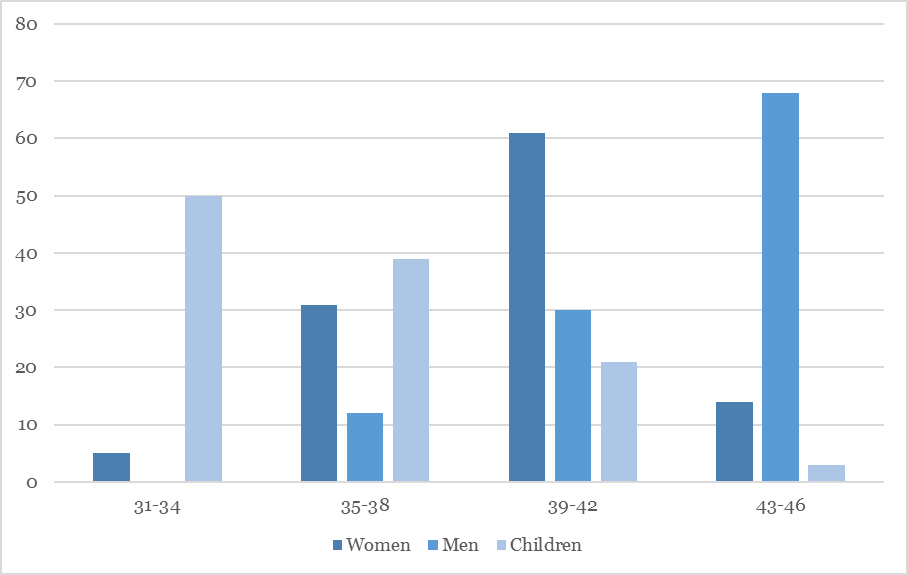
\includegraphics[width=.66\textwidth]{img/example-fig}
\caption{Frequency of shoe size in the population of men, women and children (CZSO data, Author’s calculation)}
\label{fig:freq-shoe-size}
\end{figure}


\section{Tables}

Use the floating environment \verb|table| to insert tables and in addition:
\begin{itemize}
\item for captions use the command \verb|\caption| -- is then also placed in the list of tables,
\item is used to identify the table using the command \verb|\label| (must always be after the command \verb|\caption|) -- then refer to the table in the text with the command \verb|\ref|.
\end{itemize}

\begin{table}[htbp!]

\centering
%%% Table uses the following packages:
%%% - booktabs (\toprule, \midrule, \bottomrule)
%%% - dcolumn (D column type: centered numbers aligned to
%%% decimal point
%%% Note that there are decimal points in the source code, but
%%% prints commas.

\caption{Maximum plausible estimates of models 1 and 2 (CZSO data, own processing)}\label{tab03:Nejaka}
\begin{tabular}{lrr}
\toprule
 & \multicolumn{1}{c}{\textbf{1}} & \multicolumn{1}{c}{\textbf{2}}\\
\midrule
\multirow{2}{*}{Abs} &$-$10.01*** &42.01**\\
 & (1.01) &(1.89)\\
\multirow{2}{*}{Gender (Male)} & 9.89* & 8.16\\
 & (5.98) &(8.18)\\
Height (cm) & 0.78*** &(0.12) \\
\bottomrule
\multicolumn{3}{p{.45\textwidth}}{\footnotesize \textit{Note:}:
(i) Standard errors obtained based on 500 non-parametric bootstrap iterations are given in parentheses.
(ii) * p < 0.05, ** p < 0.01, *** p < 0.001.}
\end{tabular}
\end{table}

The following tips specifically apply to \textbf{tables}:

\begin{itemize} %% or compactitem from package paralist

\item Never copy tables from statistical software to a thesis. Typically, 
statistical software also includes more information in tables than necessary.

\item Avoid vertical lines. Thicker horizontal lines separate the table from the 
surrounding text, including the legend, weaker horizontal lines separate the 
column headers from the table body, and the individual parts of the table from 
each other. In \LaTeX, the \texttt{booktabs} package implements this form of 
tables. If we want to significantly separate some columns from others, we insert 
a larger space between them

\item Keep the type, format and sense of the field content in a single column. 
It is not advised to enter, e.g., average and percent in the same column.

\item Avoid repeating the same field content too many times. E.g., if the column 
Variance shows the value of 0.5 in the first ten lines and 1.5 in the following 
ten lines, cancel the column. Find a different solution. E.g., one can divide 
the table to two. Alternatively, one can enter descriptive lines that inform of 
a variable value repeating in the following table section. E. g.
\emph{\uv{Variance${}=0,5$}} and below \emph{\uv{Variance${}= 1,5$}}).

\item All numbers shall have the same number of valid digits. Numbers in a table 
shall be aligned to the decimal point.

\item A table sometimes requires the use of abbreviations that do not occur 
elsewhere. Such abbreviations may be explained in the legend or notes below the 
table. Notes below the table may also be used for an explanation of the sense of 
some columns or values.

\end{itemize}


\section{Source codes} 
Algorithms, program listings and description of 
interaction with programs should be distinguished from the rest of the text. One 
possibility is to use {\LaTeX}'s \texttt{listings} package and its environment 
\texttt{lstlistings}.

In the file \texttt{makra.tex} the \texttt{code} environment is defined. Its use looks like this:
\begin{verbatim}
\begin{code}{programming-language}{description}{label-for-ref-ccmmand}
import numpy as np
    
def incmatrix(genl1,genl2):
...
\end{code}
\end{verbatim}

List of supported programming languages: \url{https://www.overleaf.com/learn/latex/Code_listing#Supported_languages}.

For example, the \ref{python-processing} listing is inserted like this:
\begin{verbatim}
\begin{code}{Python}{Sample processing using Python}{python-processing}
...
\end{code}
\end{verbatim}

\begin{code}{Python}{Sample processing using Python}{python-processing}
import numpy as np
    
def incmatrix(genl1,genl2):
    m = len(genl1)
    n = len(genl2)
    M = None #to become the incidence matrix
    VT = np.zeros((n*m,1), int)  #dummy variable
    
    #compute the bitwise xor matrix
    M1 = bitxormatrix(genl1)
    M2 = np.triu(bitxormatrix(genl2),1) 

    for i in range(m-1):
        for j in range(i+1, m):
            [r,c] = np.where(M2 == M1[i,j])
            for k in range(len(r)):
                VT[(i)*n + r[k]] = 1;
                VT[(i)*n + c[k]] = 1;
                VT[(j)*n + r[k]] = 1;
                VT[(j)*n + c[k]] = 1;
                
                if M is None:
                    M = np.copy(VT)
                else:
                    M = np.concatenate((M, VT), 1)
                
                VT = np.zeros((n*m,1), int)
    
    return M
\end{code}

However, the \texttt{listings} package and its environment \texttt{lstlisting} 
offer an almost endless number of configuration parameters, e.g. for syntax 
highlighting of programming languages (several dozen), line numbering, etc.
Examples:


\begin{itemize}
\sloppy
\item \url{https://en.wikibooks.org/wiki/LaTeX/Source_Code_Listings}
\item \url{https://www.overleaf.com/learn/latex/Code_listing#Using_listings_to_highlight_code}
\end{itemize}


\section{Typesetting of mathematics}

We type the variables in italics (\TeX{} does this in math mode itself, but 
don't forget that in the surrounding text and also turn on math mode). We place 
function names upright. For example:
$\textrm{var} (X) = \textsf{E~} X^2 - \bigl(\textsf{E~} X \bigr)^2$.

Fractions inside a paragraph (e. g. $\frac{5}{7}$ or $\frac{x+y}{2}$) they can 
be too cramped, so it's better to bet simple fractions with a slash: $5/7$, 
$(x+y)/2$.

The possibilities of \LaTeX\ for typesetting mathematics are rich, but they may 
not be sufficient in some specific situations. Therefore, American Mathematical 
Society (AMS) packages can be recommended for use. The \texttt{makra.tex} file 
loads the \texttt{amsmath}, \texttt{amsfonts} and \texttt{amsthm} packages 
by default. To penetrate their possibilities, the following will serve:

\begin{itemize}
\item Math Extension with AMS\LaTeX\ -- \url{http://ptgmedia.pearsoncmg.com/images/0321173856/samplechapter/kopkach15.pdf}
\item \url{https://www.overleaf.com/learn/latex/Aligning_equations_with_amsmath}
\item Math Mode -- \url{http://tex.loria.fr/general/Voss-Mathmode.pdf}
\item More Math into LaTeX -- \url{http://tug.ctan.org/info/Math_into_LaTeX-4/Short_Course.pdf}
\end{itemize}

Example of a numbered formula:
\begin{equation}
\mathbf{b}=(\mathbf{X}^\mathsf{T}\mathbf{X})^{-1}\mathbf{X}^\mathsf{T}\mathbf{y}
\end{equation}

Example of unnumbered formulas with functions and indexes:

$$
d_{ij}=\max_{k=1,2,\dots,n} \{d_{ik}+d_{kj}\},
$$
$$
x_{1,2}=b \pm \sqrt{\ln y}.
$$

An example of a formula as part of one paragraph is given on the example of 
supplier capacities in a mathematical model of a traffic problem, which we take 
into account using constraints:
\begin{equation}
\sum_{j=1}^n x_{ij} \le a_i, \qquad i=1,2,\dots,m\ ,
\end{equation}
\noindent
where expression $a_i$ represents capacity of $i$-th supplier.

When deriving a formula by incremental modification, the individual steps are 
usually listed on separate lines (\verb'align*' environment from the \verb|amsmath| package):

\begin{align*}
 f(x) &= (x+a)(x+b) =\\
      &= x^2 + bx + ax + ab =\\
      &= x^2 + (a+b)x + ab
\end{align*}

Example of column adjustment (\verb|eqnarray*|):
\begin{eqnarray*}
\sum_{i=1}^n x_{ij} =1, && j=1,2,\dots,n,\\
\sum_{j=1}^n x_{ij} =1, && i=1,2,\dots,n,\\
u_i + 1 - M(1 - x_{ij}) \le u_j, && i=2,3,\dots,n,\quad j=1,2,\dots,n,\\
u_i \ge 0,              && i=1,2,\dots,n,\\
x_{ij} \in \{0,1\} && i=1,2,\dots,n,\quad j=1,2,\dots,n,\\
\end{eqnarray*}
%\chapter{Bibliography management}

The template assumes the use of This template assumes the use of a bibliographic 
database in \BibTeX\ format for greater flexibility. The use of a bibliographic 
database is not a necessary condition, the standard environment 
\texttt{thebibliography} can also suffice. However, in such a case, it is 
necessary to make interventions in some files, as shown below.

\section{Use of bibliographic database}

\begin{enumerate}

\item \textbf{Package \verb'biblatex', APA-7}\\
The template uses settings via the \verb|biblatex| package to process the 
bibliographic database and also guarantees the use of the \textbf{APA-7} 
citation standard. All settings are listed in the file \texttt{biblatex-setup.tex}.

\item\textbf{Change the database name}\\
The template assumes a database stored in the file \texttt{bibliography.bib}. If 
the database has a different name, then it is necessary to change the value of 
the command parameter \verb'\bibliography' in the file \texttt{biblatex-setup.tex}.

\item\textbf{Change citation style}\\
By default, in-text citations are given in a combination of last name and year 
(Harvard style). You can switch to references by number by changing the 
file \nolinkurl{biblatex-setup.tex}, where the comment character in the lines is 
canceled:
\begin{verbatim}
% ,citestyle=numeric-comp
...
%\makeatletter
%\RequireBibliographyStyle{numeric}
%\makeatother
\end{verbatim}

\item \textbf{Using the popular citation manager Zotero}:
\begin{enumerate}
\item more information -- \href{https://www.zotero.org/}{homepage}, \href{https://knihovna.vse.cz/citace/nastroje/zotero/}{information from the VŠE Library}
\item Installation -- \url{https://www.zotero.org/download/}
\item Installing the browser connector -- Firefox, Chrome, Edge, Safari
\item Better BibTeX for Zotero extension -- \url{https://retorque.re/zotero-better-bibtex/}:
 \begin{enumerate}
 \item Download the .xpi file
 \item And then \texttt{Tools--Add-ons--Install Add-on From File}
 \end{enumerate}
\item \href{https://formadoct.doctorat-bretagneloire.fr/zotero_workshop/latex}{Zotero workshop or Zotero\&{}\LaTeX\ step by step}
\end{enumerate}
\end{enumerate}


\section{Use of the environment \texttt{thebibliography}}
\begin{enumerate}
\item In the file \texttt{makra.tex} at the beginning delete these lines:
\begin{verbatim}
%%% Nastavení pro použití samostatné bibliografické databáze.
%%% Settings for using a separate bibliographic database.
\input biblatex-setup
\end{verbatim}

\item In the file \texttt{bibliography.tex} delete the line 
\verb'\printbibliography' and remove the comment flag in the next section 
containing the environment \texttt{thebibliography.}

\item Individual items \verb\bibitem\ must be compiled according to the APA-7 
standard. Instructional examples are available for example here: 
\url{https://knihovna.vse.cz/citace/priklady/?norm=apa}. 
\end{enumerate}


\section{How cite in the text}
\begin{center}
\begin{tabularx}{\textwidth}{l@{~~$\longrightarrow$~~}X}
\verb|\parencite{Cermak2018}|&\parencite{Cermak2018}\\
\verb|\parencite{Hladik2018,Jasek2018}|&\parencite{Hladik2018,Jasek2018}\\
\verb|\parencite[chap. 3]{Pecakova2018}|&\parencite[chap. 3]{Pecakova2018}\\
\verb|\parencite{Furtuna2023}|&\parencite{Furtuna2023}\\
\end{tabularx}
\end{center}

%\chapter{PDF/A format}

Electronic form of final
work must be submitted in PDF/A format level 1a or 2u. They are
PDF profiles that determine which PDF properties are allowed to use
to make the documents suitable for long-term archiving and further automatic
processing. Next we will deal with level 2u, which we bet on \LaTeX{}.

The most important requirements of PDF/A-2u include:

\begin{itemize}

\item All fonts must be built into the document. They are not allowed
links to external fonts.

\item Fonts must contain a ToUnicode table that defines the conversion from encoding
characters used inside a Unicode font. This makes it possible from the document
reliably extract text.

\item The document must contain metadata in XMP format and, if colored,
then also the formal specification of color space.

\end{itemize}

This template uses the {\ tt pdfx} package, which \LaTeX{} can set up
to meet the requirements of PDF/A. Metadata in XMP is generated automatically by
information in the file {\ tt thesis.xmpdata} (you can refer to the generated file
see in {\ tt pdfa.xmpi}).

The correctness of PDF/A can be checked using an online validator: \url{https://www.pdf-online.com/osa/validate.aspx/}.

If the file is not valid, common causes include less use
common fonts (which are inserted only in bitmap format and/or without
unicode tables) and embedding images in PDF, which are standard in themselves
PDF/A do not meet.

This is likely to be the case for images created by many different programs.
In this case, you can try to convert the image to PDF/A using
GhostScript, for example, as follows:

\begin{verbatim}
        gs -q -dNOPAUSE -dBATCH
           -sDEVICE=pdfwrite -dPDFSETTINGS=/prepress
           -sOutputFile=vystup.pdf vstup.pdf
\end{verbatim}

% \include{...}
% \include{...}

{%
\pagestyle{fancyx}

\chapter{Benford's Law Background and Applicability}

Benford's Law describes a particular behaviour of digits in a number. The lowest digits (such as 1 or 2) are most likely to occur in the first and second positions within a number (labelled as significant digits), their distribution approaches logarithmic distribution, its depiction of the law is shown latter in figure \ref{fig:FL} and the approximate relative frequencies described by formula \ref{BZ-general_first}. \cite{Cerqueti2202,Hronova2023,Newcomb1881}



While this is very useful for validation and fraud detection in many areas, it's theoretical validity still has not yet been proven even though there has been some explanations put forward. %\cite{Hronova2023,Cerqueti2202} introduction 
It has been demonstrated that this behaviour is common for numbers generated by various methods, including random linear combinations, aggregation of different datasets or random selection from such, and processes arising from multiplication (such as geometric series or exponential growth). Such numbers can be found in all fields of science, including census data, stock prices or the number of seconds between earthquakes. \cite{Hronova2023,kossovsky2014benford, Cerqueti2202} %section 1-15 

Benford's law also assists in understanding the discrepancy between the perception of randomness in numbers and the actuality. Many individuals hold the notion that numbers are distributed evenly across numerous datasets, or that repetition is minimal. This is exemplified by students being required to write out random numbers as part of an experiment - without prior knowledge of this law, it is very hard to write out random numbers that are actually random. Or accountants rounding off numbers as a part of their computations. \cite{kossovsky2014benford} % section 25, strana 8é, druhá polovina 
%This is also why various manual manipulations of numbers can be identified with high accuracy by BL.

The compliance of our data to the law can be expected when only minimal conditions are met. Then the conformity can be tested. This makes the law good for detecting presence of any fraud or various manual manipulations of numbers with high accuracy. \cite{kossovsky2014benford, Cerqueti2202,kossovsky2014benford} 

\section{History}

This section will describe the historical development of this phenomenon, demonstrating that in fact Frank Benford was not the first to identify this principle. And then we shall describe some of its initial applications. \cite{kossovsky2014benford,Hronova2023}

\subsection{Simon Newcomb (1835-1909)}

The notable Canadian-American astronomer and mathematician lived in the second half of the 19th century. And although he was recognized for his work in astronomy and physics, few people have noticed his article \emph{\uv{Note on the Frequency of Use of the Different Digits in Natural Numbers}}, where he had described the regularity in the occurrence of the first digits of a number, later known as Benford's law. He demonstrates this phenomenon by calculating the relative frequencies of occurrence of the first and second digits as noted in equations \ref{BZ-general_first} and \ref{BZ-general_second}. The behaviour of the remaining digits was only described by words not by equations. \cite{kossovsky2014benford, Newcomb1881, Hronova2023}  

\subsection{Frank Benford (1883-1948)}

Frank Benford, after whom the law was named, lived at the turn of the 19th and 20th centuries, he was an American mathematician, physicist and electrical engineer, but he also held up to 20 patents in the field of optical devices. He was unaware of Newcomb's earlier paper on the frequencies of natural numbers when he published his much longer paper \emph{\uv{The Law of Anomalous Numbers}}. \cite{kossovsky2014benford, Hronova2023}

In contrast to Newcomb, Benford sought to further test the validity of the rule. Thus, he compared 20 large datasets of different data types and systematically recorded the results of these tests. However, it was not without flaws. For instance, it lacked an accurate mathematical description of the phenomenon, and some of his assumptions regarding the origin of the numbers were also unsubstantiated. \cite{kossovsky2014benford, Hronova2023}

His work was preceded by the famous story of the logarithmic tables - he saw that the tables had worn pages only at the beginning, but were as good as new at the end, as saw Newcomb earlier, which made them both think about this phenomenon. Probably, those who used them most often needed to know the value of the lower numbers in their calculations more often than of the higher values.  \cite{Hronova2023}

\subsection{Theodore Preston Hill}

It is also worth mentioning Theodore Preston Hill, who, relying on Benford's work, proved the theory of mixed distributions in 1995 and added the necessary mathematical proofs. \cite{kossovsky2014benford} % section 25, strana 80, konec  {\color{blue}(zdroj? dočíst!)} 

\subsection{The first uses of BL in practice}  

In 1972, Hal Varian, then a master's student at the University of California at Berkley, came up with the idea of using Benford's law to detect faulty data in economics. This is the first documented use of BL. \cite{kossovsky2014benford} %section 25, strana 79

He worked for a real estate agency where he found a bug in a program that was used for running simulations. So he started thinking about detecting faulty data - how to differentiate data that is \emph{genuine} from flawed data in general. He had learned about BL. After a successful application, he wrote that Benford's Law was almost to the point of being \emph{\uv{numerological}}, since it was not as strongly mathematically supported at the time as it is today. He drew on practical results that suggested that the application was valid. \cite{kossovsky2014benford} %section 25

The first person to use the BL in a scientific paper was Charles Carslaw of the University of Canterbury in New Zealand in 1988. It was applied to some data from finance and accounting. He looked at how the earnings figures for New Zealand companies came close to the theoretical proportions of BL. It showed how, contrary to the law of the last digits, %\textcolor{blue}{(doplnit presnou zkratku co budu pouzivat)}
earnings and income are often rounded to multiples of powers of 10 - as well as the losses and expenses. \cite{kossovsky2014benford} %section 25, strana 80 

The 1990s then saw the addition of many more publications %notably by Mark Nigrini, C. W. Christian, S. Gupta and many others, who
introducing the first forensic methods of how to use BL to detect manipulation or fraud. \cite{kossovsky2014benford} %section 25, strana 80 

Since then this law is nowadays used as a standard test for many tax departments worldwide. Usually in the form of a routine test where the first digits are compared to see how they are distributed across the entire dataset. Often, it is discovered that the digits are distributed evenly if the data is artificially created or has been poorly manipulated. It is also used in accounting, auditing and other financially oriented industries as well as in other fields with risk of data fraud. \cite{kossovsky2014benford} % section 26, strana 81 

\section{Applicability of Benford's Law}

The law does not put many conditions on the data that will be analysed, yet there are some that must be met for reliable results. The following will be discussed in this section. 

\subsection{Correct usage}

When using Benford's Law to detect intentional fraud or data manipulation, the complete dataset is used, rather than a subset. Additionally the dataset must satisfy conditions other than those mentioned in the previous chapters. The dataset should be large enough - for datasets with less than 100 observations, BL analysis is not recommended. %\cite{kossovsky2014benford} % section 26, strana 82
Only non-negative data should be used for an analysis. For use in auditing, it is also recommended to eliminate small numbers, values less than, for example, 50, but that the portion removed be less than $10\%$. In addition, values that represent totals, summations, etc. should not be included if came from the same sample. \cite{kossovsky2014benford} % section 27, strana 88 

When detecting similar errors, it is often not enough to look at the distribution of the first digits only. It is advised to look at the last two digits to detect rounding. For a comprehensive analysis, \citeauthor{kossovsky2014benford} recommends a nine-step procedure:

\begin{figure}[h]
    \centering
    \label{fig:enter-label}
\begin{enumerate}
    \item First-digits distribution
    \item Second-digits distribution
    \item Combination of the first-two-digits distributions
    \item Combination of the first-three-digits distributions
    \item Combination of the last-two-digits distributions 
    \item Examination of first-order digital development
    \item Examination of second-order digital development
    \item Value repetition test
    \item Summation test   
\end{enumerate}
    \source{ \citeauthor{kossovsky2014benford}, \citeyear{kossovsky2014benford}}
\end{figure}

\subsection{Varying results from the expected distribution}

It is advised to generally focus on deviations from the theoretical distribution according to a given BL variation, specifically on the significantly higher values for the frequency of occurrence for a given digit. In graphical representation, these can be represented as spikes. There is minimal interest in the reduced frequencies, as any suspicious activity is likely to manifest itself through increased frequencies - when counting frequencies, an increase in one digit is much more detectable, with all other frequencies dropping slightly. \cite{kossovsky2014benford} % section 26, strana 85 

\begin{koment}
    grafický příklad jak vypadá hrot jakožto odchylka od konformity s BZ - pokud nebudu mít nic svého, Kossovsky strana 83. Potom i další ukázky podivných situací.
\end{koment}

%There will always be variation, because few datasets are $100\%$ \textit{Benfordian}.  \cite{kossovsky2014benford} % section 26, strana 84
Deviance is to be expected - but where should the line be drawn?  \citeauthor{kossovsky2014benford} suggests to distinguish between two terms: compliance and comparison. When researching the data's compliance to BL, the data is expected to follow the logarithmic distribution very closely, the focus in on detecting manipulation and if there is, if it is random or structural. For comparison the conditions are much loose. We don't assume any \textbf{prior population type (logarithmic distribution)}. For this our use, we will be assuming the data should follow the distribution and therefore observe data compliance.


% \begin{koment}
%     Pozor na stanovení N při testování pomocí chisq testu.
%     Je tam důležité odlišit, co je skutečně ta reálná populace - uvádí na příkladu, že populace mohou být sales revenue za celé čtvrtletí (57 tisíc záznamů) - unique price list, unique products... ale třeba sales revenue z malého coffee shopu bude třeba k nějaké populaci přihodit - je zde možné testovat compliance a u toho velkého vzorku ne? Nevím, jestli to chápu dobře... 

%     Pokud ten dataset existuje sám o sobě in its unique fashion, je to potom comparison, ne compliance. Compliance to bude když testujeme (za použití statistického testu) nějaký náhodný výběr. (takže třeba hlasy jen pro jednoho z kandidátů?) 

%     Pak se dal ukazují Z testy (pro jednotlivá pozorování) a pak ChiSq test pro cele. Nakonec je pak jeste zajimava smerodnatna odchylka jako measure odlisnosti. 
% \end{koment}

Next the deviations should not show signs of any systematic error or pattern. Some pattern may emerge by rounding numbers for example. The practice of rounding data is prevalent in the context of accounting, where values ending in 00 or 50 are frequently observed. This rounding process, which is often employed to streamline computations, can give rise to manipulation of higher orders, while being harmless in context. The prevalence of these values in practice is substantiated by empirical evidence. %\cite{kossovsky2014benford} %section 27, strana 92
However, such manipulations are unacceptable in, for example, electoral statistics, where votes simply cannot be rounded.
\cite{kossovsky2014benford}

\begin{koment}
    * insert příklad z analýzy volebních výsledků v Rusku, kde se zaokrouhlovalo, nebo odkaz na vyssi kapitolu kde se k tomu snad dostanu * 
\end{koment}

There are also numbers that someone must have made up at some point, in accounting, donations are a good example. That is a number that someone has determined. Just as, for example, prizes. Such numbers does not follow BL and will show high degrees of deviations. \cite{kossovsky2014benford}

Alternatively, the validity of BL can be influenced by changed external situations in regards to the data itself. In instance, how does sales data follow BL distribution when they have been affected by the pandemic in 2020? This has been answered by \citeauthor{Hronova2023} in \citeyear{Hronova2023}. Changes like this should be taken account and analysis should be adapted accordingly.



\chapter{Methods and Theoretical Background}

This chapter explains the methods, discusses the underlying theory, and outlines key assumptions. 

\section{Benford's Law Formulation}

The relative frequency of a leading digit approaches 

\begin{equation}
    \label{BZ-general_first}
\text{P(} X = d_i\text{)}= \log_{10}(1+1/d_i)
\end{equation}

where $d_i \in \{1,\dots,9\}$ for first digit law and $d_i \in \{10,\dots,99\}$ for the first-two digits law or even $d_i \in \{100,\dots,999\}$ for the first-three digits law. For other values (negative $d_i$) the probability is 0. When plotted, it resembles nice logarithmic distribution, as seen on figure \ref{fig:FL}.  \cite{Cerqueti2202,Hronova2023,Newcomb1881}

\begin{figure}[h]
    \centering
    \caption{Theoretical frequencies of the first leading digits}
    \label{fig:FL}
    \pgfplotsset{width=8.5cm,compat=1.18}
        \begin{tikzpicture}
        \definecolor{clr1}{RGB}{00,152,129} 
            \begin{axis}[
                ybar,
                bar width=.4cm,
                enlargelimits=0.1,
                ylabel={relative frequency},
                xlabel={$d_i$},
                symbolic x coords={1,2,3,4,5,6,7,8,9},
                xtick=data,
                ]
            \addplot coordinates {(1,0.3010) (2,0.1761) (3, 0.1249) (4,0.0969) (5,0.0791) (6,0.0669) (7,0.0580) (8,0.0512) (9,0.0458)};
            \end{axis}
        \end{tikzpicture}
    \source{ and processing: author}
\end{figure}

The first leading digit is the one found at the highest order and is non-zero. In the case of the number 124.857, the first digit would be 1, whereas for the number 0.03958, the first digit would be 3. According to Benford's law of the first digit, the theoretical frequencies correspond to the equation \ref{BZ-general_first}, indicating that the digit 1 occurs in the first position with a probability of 0.3, the digit 2 with 0.18, and so forth, with the digit 9 occurring with a probability of only 0.046. For all first digits from 1 to 9, see the BL column in the table in the Figure \ref{table:BL-table}.
%Compliance to this distribution is the first step in the nine-step procedure recommended by \citeauthor{kossovsky2014benford}, as mentioned in section \ref{correct_usage}.

As can be seen in the graph \ref{fig:FL}, the distribution is heavily skewed in favour of the lowest digits. As we move to the second (figure \ref{fig:second-digit-law}) and higher digits, this skew will flatten out significantly until there is no difference between the digits.  \cite{kossovsky2014benford}

This can be described by 

\begin{equation}
    \label{BZ-general_second}
    P(d) = \sum\limits_{k=1}^{9} \log_{10}\left( 1+\frac{1}{10k+d}\right), \quad \text{for } d = 0,1,\dots,9
\end{equation}

as mentioned by \citeauthor{Hronova2023} in \citeyear{Hronova2023}, assuming the independent occurence of the second leading digits. 

\begin{figure}[h]
    \centering
    \caption{Theoretical frequencies of the second leading digits}  
    \label{fig:second-digit-law}
        \pgfplotsset{width=8.5cm,compat=1.18}
            \begin{tikzpicture}
            \definecolor{clr1}{RGB}{00,152,129} 
                \begin{axis}[
                    ybar,
                    bar width=.4cm,
                    ymin=0.015,
                    ytick={0.12, 0.08, 0.04},
                    enlargelimits=0.1,
                    ylabel={relative frequency},
                    xlabel={$d$},
                    symbolic x coords={0, 1,2,3,4,5,6,7,8,9},
                    xtick=data,
                    yticklabel style={/pgf/number format/fixed, /pgf/number format/precision=2},
                    ]
                \addplot coordinates {(0,0.12) (1,0.114) (2,0.109) (3, 0.104) (4,0.10) (5,0.097) (6,0.093) (7,0.09) (8,0.088) (9,0.085)}; %[clr1,fill=clr1,opacity=0.55]
                \end{axis}
            \end{tikzpicture}
    \source{ and processing: author}
\end{figure}

The distribution for the second digits is less skewed than that of the first leading digits. 
%Compliance to this distribution is the second step in the nine-step procedure recommended by \citeauthor{kossovsky2014benford}, as mentioned in section \ref{correct_usage}.
Coming to the third leading digit, the relative frequencies start to be close to equal as seen on figure \ref{fig:third-digit-law}. \cite{kossovsky2014benford}

This is explained by the following equation 

\begin{equation}
    P(d) = \sum\limits_{d_1=1}^{9} \sum\limits_{d_2=1}^{9} \dots \sum\limits_{d_{k-1}=1}^{9}   \log_{10}\left( 1+\frac{1}{\sum\limits_{i=1}^{k} d_i \cdot 10^{k-i} }\right), \quad \text{for } d_k = 0,1,\dots,9 
\end{equation}

describing third and following position relative frequencies, again with the assumption of independence of digit occurrences. And \uv{\emph{the Benford distribution converges to a uniform
multinomial distribution}} as put in \citeauthor{Hronova2023} in \citeyear{Hronova2023}. 

\begin{figure}[ht!]
    \centering
    \caption{Theoretical frequencies of the third leading digits}  
    \label{fig:third-digit-law}
    \pgfplotsset{width=8.5cm,compat=1.18}
        \begin{tikzpicture}
        \definecolor{clr1}{RGB}{00,152,129} 
            \begin{axis}[
                ybar,
                bar width=.4cm,
                ymin=0.015,
                ytick={0.09, 0.06, 0.03},
                enlargelimits=0.1,
                ylabel={relative frequency},
                xlabel={$d$},
                symbolic x coords={0,1,2,3,4,5,6,7,8,9},
                xtick=data,
                yticklabel style={/pgf/number format/fixed, /pgf/number format/precision=2},
                ]
            \addplot coordinates {(0,0.1018) (1,0.1014) (2,0.1010) (3, 0.1006) (4,0.1002) (5,0.0998) (6,0.0994) (7,0.0990) (8,0.0986) (9,0.0983)};
            
            \end{axis}
        \end{tikzpicture}
    \source{ and processing: author}
\end{figure}

So for digits in the last position, the distribution is expected to be very close to, if not uniform. 


\subsection{Uniform discrete distribution}

Distribution, where every value of a random discrete variable $X$ has the same probability, is named the uniform distribution. It has many uses, eg., can be used to select a value from a set, when all values have the same probability. The probability is 

\begin{equation}
\begin{aligned}
    P(d) &= \frac{1}{n}, &\qquad d=0,1,\dots,n \\
         &= 0,           &\qquad \text{else.}
\end{aligned}
\end{equation}


If digits in a long enough number were distributed equally, according to the uniform distribution, the distribution would look like in figure \ref{fig:BZ-uniform}, where all digits have the probability of 0.1. \cite{kossovsky2014benford, Hronova2023, Marek2024}

\begin{figure}[ht!]
    \centering
    \caption{Theoretical frequencies of digits under uniform distribution}  
    \label{fig:BZ-uniform}
    \pgfplotsset{width=8.5cm,compat=1.18}
        \begin{tikzpicture}
        \definecolor{clr1}{RGB}{00,152,129} 
            \begin{axis}[
                ybar,
                bar width=.4cm,
                ymin=0.015,
                ytick={0.09, 0.06, 0.03},
                enlargelimits=0.1,
                ylabel={relative frequency},
                xlabel={$d$},
                symbolic x coords={0,1,2,3,4,5,6,7,8,9},
                xtick=data,
                yticklabel style={/pgf/number format/fixed, /pgf/number format/precision=2},
                ]
            \addplot coordinates {(0,0.1) (1,0.1) (2,0.1) (3, 0.1) (4,0.1) (5,0.1) (6,0.1) (7,0.1) (8,0.1) (9,0.1)};
            \end{axis}
        \end{tikzpicture}
    \source{ and processing: author}
\end{figure}

\subsection{The Scale Invariance Principle of Benford's Law}

Given a dataset that behaves according to BL, changing units (multiplying the whole dataset by the same constant) will still behave according to BL. Any arithmetic operation applied to the whole dataset does not change the underlying BL distribution. \cite{kossovsky2014benford, Hronova2023} %section 23 The Scale Invariance Principle 

\subsection{Digital Development Pattern} \label{DDPattern}

Digital development pattern refers to the way distributions of digits evolve across different ranges of data. This pattern is observed in all random data sets, whether they follow Benford's Law or not. The pattern shows how the distribution of digits changes from lower to higher values of the data range. 

This pattern can only be seen when the data range is partitioned along integral powers of ten, such as (0.1, 1), (1, 10), (10, 100), etc. The pattern shows increasing skewness as you move from the left to the right of the data range. For smaller values, digit distributions are more equal. In the centre, the distribution becomes more logarithmic. For larger values, the distribution becomes highly skewed in favour of low digits. \cite{kossovsky2014benford}


\subsection{Applicability of Benford's Law}

The law does not impose many conditions on the data that will be analysed, yet some must be met for reliable results. This section will discuss the following. 

\subsubsection*{Order of Magnitude of Variability (OMV)}

\citeauthor{kossovsky2014benford} notes that for data to behave according to BL, its value range should be wider, rather than narrow. He describes a measure, Order of Magnitude of Variability (OMV), as 

\begin{equation}
    OMV = \log_{10}(\text{90th percentile}) - \log(\text{10th percentile}) > 3 
    \label{OMV}
\end{equation}

and recommends it should be larger than 3. In practice, this means that our data should spread all the way from 1 to 10000 or more for consistent results. If we were to use data with lower OMV than recommended, we would get results that look fraudulent, while being genuine - data like this has higher probabilities of type I error when testing for compliance with BL.

However, election data, analysed in this thesis, should comply with the BL distribution either way. For our purposes, we will focus on a more liberal measure, the Order of Magnitude OOM, that is defined as

\begin{equation}
    OOM = \log_{10}(\text{max}) - \log(\text{min}) > 3. 
    \label{OOM}
\end{equation}

This measure works best when outliers are removed. When rejected, the convergence of BL to the uniform distribution is flawed and specific frequencies for digits on given positions should rather be used. \cite{kossovsky2014benford}
 
\subsubsection*{Correct usage} 

The compliance of our data with the law can be expected when only minimal conditions are met. Then the conformity can be tested. This makes the law good for detecting the presence of fraud or various manual manipulations of numbers with high accuracy. \cite{kossovsky2014benford, Cerqueti2202,kossovsky2014benford} 

When using Benford's Law to detect intentional fraud or data manipulation, the complete dataset is used, rather than a subset. Additionally, the dataset must satisfy conditions other than those mentioned in the previous chapters. The dataset should be large enough - for datasets with less than 100 observations, BL analysis is not recommended. %\cite{kossovsky2014benford} % section 26, strana 82
Only non-negative data should be used for analysis. For use in auditing, it is also recommended to eliminate small numbers, values less than, for example, 50, but that the portion removed be less than $10\%$. In addition, values that represent totals, summations, etc., should not be included if they come from the same sample. \cite{kossovsky2014benford} % section 27, strana 88 

\subsubsection*{Varying results from the expected distribution}

It is generally advisable to focus on deviations from the theoretical distribution in a given BL variation, specifically on the significantly higher values for the frequency of occurrence of a given digit. In graphical representation, these can be represented as spikes. There is minimal interest in the reduced frequencies, as any suspicious activity is likely to manifest itself through increased frequencies - when counting frequencies, an increase in one digit is much more detectable, with all other frequencies dropping slightly. \cite{kossovsky2014benford} % section 26, strana 85 

% \begin{koment}
%     grafický příklad jak vypadá hrot jakožto odchylka od konformity s BZ - pokud nebudu mít nic svého, Kossovsky strana 83. Potom i další ukázky podivných situací.
% \end{koment}

%There will always be variation, because few datasets are $100\%$ \textit{Benfordian}.  \cite{kossovsky2014benford} % section 26, strana 84

Deviance is to be expected, but where should the line be drawn?  \citeauthor{kossovsky2014benford} suggests distinguishing between two terms: compliance and comparison. When researching the data's compliance with BL, the data is expected to follow the logarithmic distribution very closely, the focus is on detecting manipulation, and if there is, whether it is random or structural. For our use, we assume the data follows the distribution and therefore observe data compliance.

Next, the deviations should not show signs of any systematic error or pattern. Some pattern may emerge by rounding numbers, for example. The practice of rounding data is prevalent in the context of accounting, where values ending in 00 or 50 are frequently observed. This rounding process, which is often employed to streamline computations, can give rise to manipulation of higher orders while being harmless in context. Empirical evidence supports the prevalence of these values in practice. 
However, such manipulations are unacceptable in, for example, electoral statistics, where votes simply cannot be rounded.
\cite{kossovsky2014benford} %\cite{kossovsky2014benford} %section 27, strana 92

Alternatively, the validity of BL can be influenced by changed external situations in regards to the data itself. For instance, how does sales data follow BL distribution when affected by the pandemic in 2020? This has been answered by \citeauthor{Hronova2023} in \citeyear{Hronova2023}. Changes like this should be taken into account, and analysis should be adapted accordingly.


% \section{Descriptive statistics}

% % \subsection{Miry polohy}

% \subsection{Expected value}

% For discrete variables: 
% \begin{equation}
%     % E(X) = \frac{1}{n} \sum \limits_{i=0}^{n} X_i
%     E(X) = \sum \limits_{i=0}^{n} x_i P(X=x_i)
% \end{equation}

% For continuos variables: 
% \begin{equation}
%     % E(X) = \frac{1}{n} \sum \limits_{i=0}^{n} X_i
%     E(X) =  \int \limits_{-\infty}^{\infty} x f(x) dx
% \end{equation}

% \cite{Marek2024} 

% % \subsection{Miry variability}

% \subsection{Variance}

% Variance is a measure of variability, its square root is the standard deviation. 

% \begin{equation}
%     D(X) = E(X^2) - E(X)^2 = E\{[X-E(X)]^2\}
% \end{equation}

% \begin{equation}
%     \text{sd}(X) = \sqrt{D(X)} 
% \end{equation}

% \cite{Marek2024}


% \subsection{Correlation}

% Correlation or correlation coefficient describes the relationship or dependency between two variables. It is defined as 

% \begin{equation}
%     \rho(X,Y) = \frac{\text{cov}(X,Y)}{\sqrt{D(X)D(Y)}} 
% \end{equation}

% and cov$(X,Y)$ is covariance and is defined as: 

% \begin{equation}
%  \text{cov}(X,Y) = E(X-E(X), Y-E(Y)) = E(XY)-E(X)E(Y). 
% \end{equation}

% Covariance and correlation both contain the same information, but the correlation coefficient in a given range: $\rho(X,Y) \in \langle-1,1\rangle$. The value -1 denotes a very strong negative dependency of X and Y variables, 0 is no relationship and 1 is a strong positive dependency of the variables. 

% \cite{Marek2024}

\section{Selected relevant distributions}

\subsection{Logarithmic distribution}

\subsection{Uniform distribution}

\begin{koment}
    Popisuje chovani last digits, vlastne s pribyvajicimi digits v cisle BL k tomuto rozdeleni konverguje. Tvrdi to Kossovsky, Hronova i ten pan co analyzoval psychologii lidi. Ale je nejaky dukaz? 
\end{koment}

\newpage

\subsection{Exponential distribution}

\begin{koment}
    why is it relevant? 
\end{koment}

Describing the distance between independent events in time, the exponential distribution is \textcolor{blue}{...} with the key property in being memoryless. PDF is one of the defining features of a random variable $X$, and for variables coming from an exponential distribution is defined as: 

\begin{equation}
    f(x;\lambda) = \lambda e^{-\lambda x} \quad \text{for } x \ge 0 
\end{equation}

where $\lambda$ is the rate parameter. \cite{Marek2024}

\begin{figure}[h]
    \centering
    \caption{Exponential Distribution $\lambda = 1$}
    \label{fig:Exp1}
    \begin{tikzpicture}
        \begin{axis}[
            domain=0:5,
            samples=100,
            axis x line=middle,
            axis y line=middle,
            xlabel={$x$},
            ylabel={$f(x)$},
            xtick={1,2,3,4,5},
            ytick={0.25, 0.5, 0.75,1},
            grid=major,
            grid style={dashed, gray!20},
            enlargelimits=true,
            %title={Exponential Distribution: $\lambda e^{-\lambda x}$ for $\lambda = 1$}
        ]
        \addplot[blue, thick] {exp(-x)};
        \end{axis}
    \end{tikzpicture}
    \source{ and processing: author}
\end{figure}

\begin{koment}
    Jak se exponencialni rozdeleni tyka BL? 

    Benfordovo rozdeleni muze pripominat exponencialni rozdeleni, proto bych mela popsat, jak to rozdeleni vypada, nakreslit nejaky pekny grafik a popsat co dela parametr lambda. Mozna by se hodil nejaky pekny priklad pouziti? 

    Mozna me jeste napada, jestli sem nenapsat co je to rozdeleni, frekventisticka definice pravdepodobnosti (since pocitam relativni frekvence vyskytu cislic na dane pozici a prirovnavam to k pravdepodobnostem) 
\end{koment}

Kdyz porovname exponencialni rozdeleni a rozdeleni podle benfordova zakona, narazime na dve vyrazne odlisnosti 
Benforduv zakon je diskretni (relativni frekvence pro jednotlive cislice), exponencialni rozdeleni je spojite. Dal, Benforduv zakon ma vetsi tails (jestli se tomu da vubec tak rikat pro diskretni rozdeleni), zatimco exponencialni rozdeleni ma tails velmi male. Pri zvoleni parametru, aby si byla rozdeleni blizka, vidime, jak jsou si odlisna. 

\begin{figure}[h]
    \centering
    \caption{Porovnani BL a Exp(0.45)}
    \label{fig:Exp0.45aBL}
    \begin{tikzpicture}
        \begin{axis}[
            width=13cm,  % Set the width of the plot
            height=8cm,  % Set the height of the plot
            domain=0:9,
            samples=100,
            axis x line=middle,
            axis y line=middle,
            xlabel={$x$},
            ylabel={$f(x)$},
            xtick={1,2,3,4,5,6,7,8,9},
            yticklabel style={/pgf/number format/.cd, fixed, precision=2}, 
            %ytick=\empty, 
            grid=major,
            grid style={dashed, gray!20},
            enlargelimits=true,
            %title={Porovnani BL a Exp(0.45)},
            legend style={draw=none, font=\small, cells={anchor=west}},
            legend pos=north east
        ]
        \addplot[blue, thick] {0.45*exp(-0.45*x)};
        \addlegendentry{$\lambda e^{-\lambda x}$}
        \addplot+[red, only marks, mark=*, mark size=2]
            coordinates {
            (1,0.3010) 
            (2,0.1761) 
            (3, 0.1249) 
            (4,0.0969) 
            (5,0.0791) 
            (6,0.0669) 
            (7,0.0580) 
            (8,0.0512) 
            (9,0.0458)
            };
        \addlegendentry{$\log_{10}(1 + \frac{1}{x})$}

        \end{axis}
    \end{tikzpicture}
    \source{ and processing: author}
\end{figure}


% %It is a non negative function, which sum equals to one. 

% For continuos variable is it defined as 

% \begin{equation}
%     P(x_1 \le X \le x_2) = \int\limits_{x_1}^{x_2} f (x) dx
% \end{equation}

% The distribution function is defined as 

% \begin{equation}
%     F(x) = P(X \le x), \quad \forall x \in R
% \end{equation}

% \begin{equation}
%     F(x) = \int\limits_{-\infty}^{x} f (t) dt, \quad -\infty <x<\infty
% \end{equation}

% \begin{koment}
%     neklesajici, v $-\infty$ je 0, v $\infty$ je 1

%     vymyslet jak to pojmout a propojit? 
% \end{koment}


\section{Hypothesis testing}

Hypothesis testing is a fundamental framework used to test a theory about a population based on a sample by comparing two hypotheses in statistics at the given \textbf{level of significance}. The tested hypothesis is the \textit{null hypothesis} $H_0$. An alternative to this, usually a negation, always a disjunction, is the \textit{alternative hypothesis} $H_1$. 

\begin{equation}
    H_0: \theta = \theta_0 \qquad \qquad H_1:  \theta \ne \theta_0
\end{equation}

In this case, we test whether the parameter $\theta$ is $\theta_0$ coming from a sample data. To test this assumption, a sample from the population is taken and analysed.  

Given the nature of the test, we select the \textbf{test statistic}. Its value comes from the sample of data and can fall into two sets. One, where its values are not in conflict with the null hypothesis, the acceptance region $V_\alpha$, and the other, where the values conflict with the null hypothesis, the \textbf{rejection region} $W_\alpha$. The \textbf{critical value} is the boundary for rejecting the null hypothesis. In the end, it is decided based on the critical value and test statistic which hypothesis is rejected, but neither accepted. Or the \textbf{p-value} is computed and compared to the level of significance. \cite{Mala2024, Marek2024}

\subsubsection*{Type I. and Type II. errors}

Working with sample data, there are two specific kinds of errors, and the probability of one influences the probability of the other. 

\textbf{Type I. error} $\alpha$ is the given level of significance, and it is the probability of rejecting the null hypothesis if the null hypothesis is correct. The $\alpha$ is usually set at 0.05. 

\begin{equation}
    \alpha = P(W_\alpha | H_0)
\end{equation}

\textbf{Type II. error} $\beta$ is the probability of not rejecting the null hypothesis if the null hypothesis is not correct. 

\begin{equation}
    \beta = P(V_\alpha | H_1)
\end{equation}

The probability $1-\beta$ is the \textbf{power of test} and denotes the probability of correct rejection of the null hypothesis. 

\subsubsection*{P-value}

The probability of obtaining a result which is as far or further from $H_{0}$ than the observed value. We reject the $H_{0}$ when  $p \le \alpha$ and we reject the $H_{1}$ when $p \ge \alpha$.

\subsection{$\chi^2$ goodness of fit test}

To check the compliance of the data to the BL, we can use the $\chi^2$ goodness of fit test. \\ This test is generally used to test whether the sample comes from an assumed population. The null hypothesis assumes the empirical distribution follows the theoretical distribution. The alternative hypothesis is the opposite. 

\begin{equation}
\begin{aligned}
    H_0&: \pi_d = p_d, \qquad d \in D\\
    H_1&: \pi_d \ne p_d
\end{aligned}
\end{equation}

$d$ comes from a set $D$, which contains all possible digits. For testing of the compliance of the first leading digits in numbers according to BL, $D = \{1,2,\dots,9\}$. $k$ is the number of digits, in this case $k = 9$.

The test statistic is given as such  

\begin{equation}
    \label{chi-sq-test}
    G= n \sum\limits_{d=1}^{9} \frac{(p_d -\pi_d)^2}{\pi_d} \qquad \qquad  G \approx \chi^2(k-1) 
\end{equation}

\begin{align*}
    \text{where } &\pi_d \text{ is the theoretical frequency under BL distribution}, \\
    &p_d \text{ is the empirical frequency from the data} \\ 
    &n \text{ is the sample size, and} \\
    &d \text{ is the corresponding digit}
\end{align*} 

as recommended in \citeauthor{Hronova2023}, \citeyear{Hronova2023} and  \citeauthor{kossovsky2014benford}, \citeyear{kossovsky2014benford}. 

There is one assumption, and that is that the sample size is large enough.  
$n \cdot \pi_d > 5$ for all $d$ (as put differently, there is enough observations for each digit). The rejection region under the null hypothesis is 

\begin{equation}
    W_\alpha = \left( \chi^2; G \ge \chi^2_{1-\alpha}(k-1) \right) = (\chi^2_{1-\alpha}(9-1), \infty)
\end{equation}

for the distribution of the first leading digit.

The test can be summed up as the larger the fraction \ref{chi-sq-test}, the poorer the fit between the empirical and theoretical frequencies.

% \begin{koment}
%     Pozor na stanovení N při testování pomocí chisq testu.
%     Je tam důležité odlišit, co je skutečně ta reálná populace - uvádí na příkladu, že populace mohou být sales revenue za celé čtvrtletí (57 tisíc záznamů) - unique price list, unique products... ale třeba sales revenue z malého coffee shopu bude třeba k nějaké populaci přihodit - je zde možné testovat compliance a u toho velkého vzorku ne? Nevím, jestli to chápu dobře... 

%     Pokud ten dataset existuje sám o sobě in its unique fashion, je to potom comparison, ne compliance. Compliance to bude když testujeme (za použití statistického testu) nějaký náhodný výběr. (takže třeba hlasy jen pro jednoho z kandidátů?) 

%     Pak se dal ukazují Z testy (pro jednotlivá pozorování) a pak ChiSq test pro cele. Nakonec je pak jeste zajimava smerodnatna odchylka jako measure odlisnosti. 
% \end{koment}

% \subsubsection*{Z test}

% This test is performed individually on a particular digit/combination, however, the false positive error (type I) is more likely for the overall test of the chi-square.

% Null hypothesis: Data obeys Benford's Law in the context of the particular digit/combination. % this individual observation obeys the benfords law ? 

% \begin{equation}
%     \label{z_test}
%     Z_d = \frac{|P_o - P_e| - 1/2n}{\sqrt{(P_e(1-P_e)/n}}
% \end{equation}

% \begin{align*}
%     \text{where } &P_o \text{ is the observed frequency of the particular digit/combination}, \\
%     &P_e \text{ is the expected Benford proportion for the particular digit/combination, and} \\ 
%     &n \text{ is the sample size}
% \end{align*} 

% We reject the null hypothesis when the $Z_d$ value is larger than $Z$ with the level of significance, $\alpha$. $Z$ refers to the Standardized Normal Distribution, a Normal distribution with mean 0 and standard deviation 1. \cite{kossovsky2014benford}

% \begin{koment}
%     Ještě se rozhoduju, jestli se mi to k něčemu nebude hodit, tak to tu zatím nechávám.  
% \end{koment}

\newpage

\section{Analysis workflow}

The analysis workflow used in this thesis can be seen in the figure \ref{fig:analysis-workflow}.  Its elements will be commented on below. 

\begin{figure}[h]
    \centering
    \caption{Analysis workflow}
    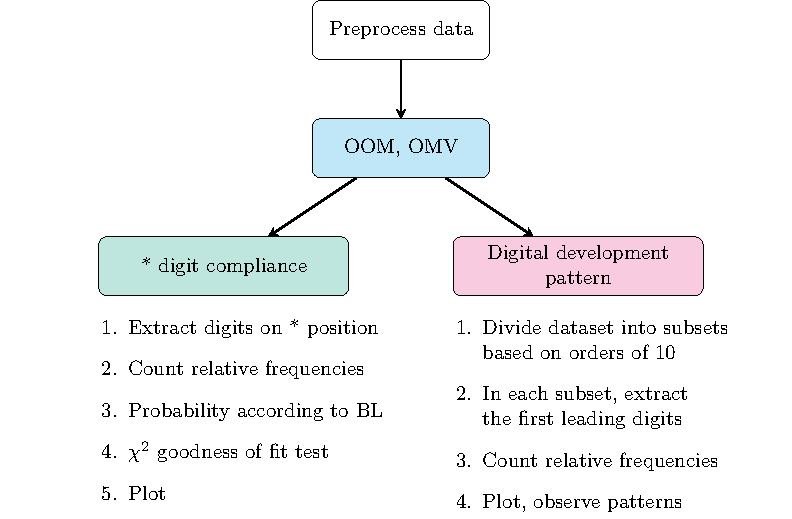
\includegraphics[width=0.9\linewidth]{BT-DT-eng/TemplateBT-DT/img/diagram.pdf}
    \label{fig:analysis-workflow}
    \source{ and processing: author}
\end{figure}

\subsubsection{Data preprocessing}

To start this process, the data is loaded into the R software. The election results for a small territory are chosen. One statistical unit is a town in the Czech Republic, a county in the USA or a polling station in Belarus. The decision for selection of the size of the region is based on individual accounting for the size of the country, total sample size and availability, so that the dataset would be suitable for the methodology of this thesis, namely the BL.

Next, the relevant variables are selected. Most important are the vote counts of the candidates and the totals. There are two candidates in the Czech elections, the USA and Belarus have two main candidates and a couple of other candidates with very few votes. The two candidates with the majority of votes are selected. 

Afterwards, the data types are changed into those that are suitable for the analysis; vote counts are typically a numerical discrete (integer) variable, and their validity is checked (control sums of the number of votes). 

\subsubsection{Order of Magnitude}

OOM measure tells us whether we can use the last digit test responsibly. If the OOM test is rejected ($OOM < 3$), we should not test compliance of the last digits or last two digits to the uniform distribution (which is the generalised BL). The relative frequencies are influenced by their position. So instead of last digits, we should take their position from the most significant digit - \_. leading digit. 

\subsubsection{Digit compliance on a given position} 

In this first and most important section, we look at how well the relative frequencies follow the BL variation. Namely, we shall focus on these positions in numbers: 

\begin{itemize}
    \item First digit 
    \item First two digits 
    \item Second digit 
    \item Third digit 
    \item Last digit
\end{itemize}

In the first digit distribution, the most famous BL is applied, as formulated in \ref{BZ-general_first} equation. The same information, but in better detail, is seen in the distribution of the first two digits. The second digit distribution, as noted by \citeauthor{Beber2012} and \citeauthor{Mebane2011}, is suitable for detecting digital fraud. Similarly, with the third digit distribution, for which the distribution starts to resemble the uniform distribution, as can be seen on \ref{fig:third-digit-law} graph. And lastly, we shall take a look at the relative frequencies of the last digits.

Firstly, the relevant digits on the given position need to be extracted. Then their relative frequency and the probability according to the BL are counted, as seen in an example table \ref{table:BL-table}. This table is used for the following testing and plotting.  

\begin{table}[h]
\centering
    \caption{The frequencies of the first leading digits and probabilities according to the BL \\the Czech presidential elections 2023}
    \begin{tabular}{c|rrrcr}
        \hline
        digit & Freq & Total & RelFreq & BL     & diff    \\ \hline
        1     & 1866 & 6320  & 0.2953  & 0.3010 & -0.0058 \\
        2     & 1090 & 6320  & 0.1725  & 0.1761 & -0.0036 \\
        3     & 811  & 6320  & 0.1283  & 0.1249 & 0.0034  \\
        4     & 621  & 6320  & 0.0983  & 0.0969 & 0.0013  \\
        5     & 492  & 6320  & 0.0778  & 0.0792 & -0.0013 \\
        6     & 434  & 6320  & 0.0687  & 0.0669 & 0.0017  \\
        7     & 368  & 6320  & 0.0582  & 0.0580 & 0.0002  \\
        8     & 302  & 6320  & 0.0478  & 0.0512 & -0.0034 \\
        9     & 336  & 6320  & 0.0532  & 0.0458 & 0.0074  \\ \hline
    \end{tabular}
    \source{: \citeauthor{CR23data}, \citeyear{CR23data}, processing: author}
    \label{table:BL-table}
\end{table}

All those distributions for given positions shall be tested by the $\chi^2$ goodness of fit test, as defined in \ref{chi-sq-test}, and then plotted with the corresponding p-value of the test. In some graphs, the p-value is labelled as unreliable, which signifies that the assumption of the test was not met (the absolute frequency of any digit was smaller than 5). 

There are also two points of view, the first on the totals of votes and the second on the dual plots with the counts for the individual candidates. This is important to see if there was an interest in manipulating one candidate more than the other. 

The distribution of the last two digits is not examined due to inconclusive results given by the nature of the data - the range is from 0 to 10000 usually, depending on the country and the examined regional level, and for some numbers the last two digits can be the whole number, so the relative frequencies do not match. 

\subsubsection{Digital development pattern} 

In this part, an accompanied indicator is examined, the digital development pattern. The expected behaviour of such is described in \ref{DDPattern}. It is not so strict; we are searching for some anomalies while also observing what part of the dataset is represented in a given range. This provides additional information on how well the data would comply with the BL. 

% \subsubsection{Correlation between selected variables}

% As \citeauthor{Lebeda2021} mentioned in their paper, observing the relationships between the valid votes and the votes for each candidate is an essential part of election analysis, so this part shall not be forgotten. It is not in the primary focus of this thesis, however, it will add a point of view in this analysis. The results from this part are just for a general picture. 

% We are searching for some patterns, a high correlation between turnout and votes for a specific candidate, or any anomalies of other kinds. Ideally, the turnout, the percentage of valid votes, should both be uncorrelated, unrelated to the share of votes of each candidate, as \citeauthor{Lebeda2021} mentioned. 

\chapter{Application on Election Data} %of Benford's Law 




\section{Czechia Presidential elections in 2023}




\section{Estonia?}

\section{Russia?}

\section{USA?}

\begin{koment}
plus jeste nejaky aktualni? treba Belorusko 2025 nebo tak 
\end{koment}
    





}

{%
\pagestyle{plain}
\chapter*{Conclusion}
\addcontentsline{toc}{chapter}{Conclusion}

In the conclusion, the author summarizes the individual conclusions, analyses 
and interpretations. It is useful if the author concludes by acknowledging the 
limits of his/her work and possibilities of continuing the topic.

\begin{koment}

    Vyznam BL pro aplikaci v digital fraud detection pro volby 

    Jednoduchost implementace 

    Ceske prezidentske volby: 
    \begin{itemize}
        \item transparentni uz jen tim, ze je k datum snadny pristup na CZSO webovych strankach 
        \item no evidence of fraud 
        \item posudek od OBSE , jen ze mame zrusit trest za pomluvu :)))
    \end{itemize}

    Americke prezidentske volby: 
    \begin{itemize}
        \item decentralizace volebniho system, dela si to kazdy stat sam, tezke kdyz chci konkretni data 
        \item no evidence of large scale fraud 
        \item posudek od OBSE
    \end{itemize}

    Beloruske prezidentske volby: 
    \begin{itemize}
        \item netransparentni
        \item multiple evidences of fraud 
        \item Voice, Zubr, Honest People dobra peace   
        \item vsichni vedi, ze v Belorusku si prezidenta proste nezvolis 
    \end{itemize}

    Limity digital detection of fraud 

    Other types of fraud

    Rozsireni (correlation among variables a tak) 

\end{koment}
}

%%% Seznam použité literatury
%%% Bibliography
%% This applies if a separate bibliographic database is used
\printbibliography[title={\bibnamex},heading={bibintoc}]

%% This is true when using thebibliography environment
%% The following can be recommended for compiling citation data:
%%     https://knihovna.vse.cz/citace/priklady/
%%     https://www.citace.com/
%\openright
%\phantomsection
%\addcontentsline{toc}{chapter}{\bibnamex}
%\begin{thebibliography}{99}
%\bibitem{Cermak2018}ČERMÁK, Radim, SMUTNÝ, Zdeněk. A Framework for Cultural Localization of Websites and for Improving Their Commercial Utilization. In:  \emph{Global Observations of the Influence of Culture on Consumer Buying Behavior} [online]. Hershey~: IGI Global, 2018, s. 206--232. ISBN 978-1-5225-2727-5. DOI: 10.4018/978-1-5225-2727-5.
%
%\bibitem{Hladik2018}HLADÍK, Milan, ČERNÝ, Michal. The Shape of the Optimal Value of a Fuzzy Linear Programming Problem. In: \emph{Fuzzy Logic in Intelligent System Design} [online]. Cancum, 16.10.2017 -- 18.10.2017. Cham~: Springer, 2018, s. 281--286. Advances in Intelligent Systems and Computing 648. ISBN 978-3-319-67136-9. DOI: 10.1007/978-3-319-67137-6\_31.
%
%\bibitem{Jasek2018}JAŠEK, Pavel, VRANÁ, Lenka, ŠPERKOVÁ, Lucie, SMUTNÝ, Zdeněk, KOBULSKÝ, Marek. Modeling and Application of Customer Lifetime Value in Online Retail. \emph{Informatics} [online]. 2018, roč. 5, č. 1. 22 s. eISSN 2227-9709. DOI: 10.3390/informatics5010002. Dostupné také z: \url{http://www.mdpi.com/2227-9709/5/1/2/pdf}.
%
%\bibitem{Pecakova2018}PECÁKOVÁ, Iva. \emph{Statistika v terénních průzkumech}. 3. přeprac. vyd. Praha~: Professional Publishing, 2018. 254 s. ISBN 978-80-88260-10-3.
%\end{thebibliography}


%%% Přílohy k práci, existují-li. Každá příloha musí být alespoň jednou
%%% odkazována z vlastního textu práce. Přílohy se číslují.
%%% Attachments to thesis, if any. Each attachment must be referenced at 
%%% least once in your own text. The appendices are numbered.
\part*{\Prilohy\thispagestyle{empty}}
\appendix
\chapter{Name of appendix}


\chapter{Additional outputs of analysis of the USA presidential election in 2024}

% \begin{figure}[h]
%     \centering
%     \caption{First digit distribution, total votes, USA 2024}
%     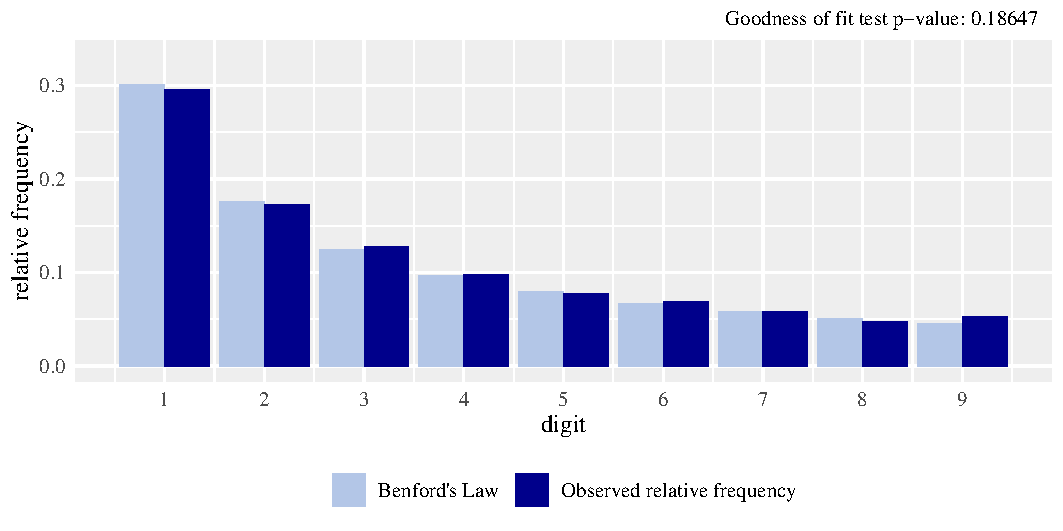
\includegraphics[width=0.99\linewidth]{BT-DT-eng/fig/USA24-both-first_digits.pdf}
%     \label{fig:USA24-both-first_digits}
% \end{figure}

% \begin{figure}[h]
%     \centering
%     \caption{First two digits distribution, total votes, USA 2024}
%     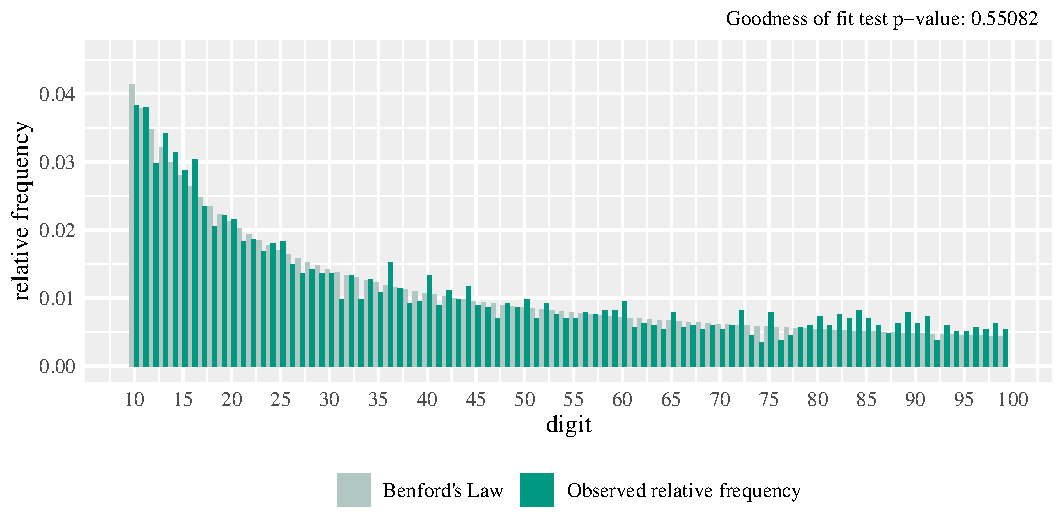
\includegraphics[width=0.99\linewidth]{BT-DT-eng/fig/USA24-both-first_two_digits.pdf}
%     \label{fig:USA24-both-first_two_digits}
% \end{figure}

% \begin{figure}[h]
%     \centering
%     \caption{Second digit distribution, total votes, USA 2024}
%     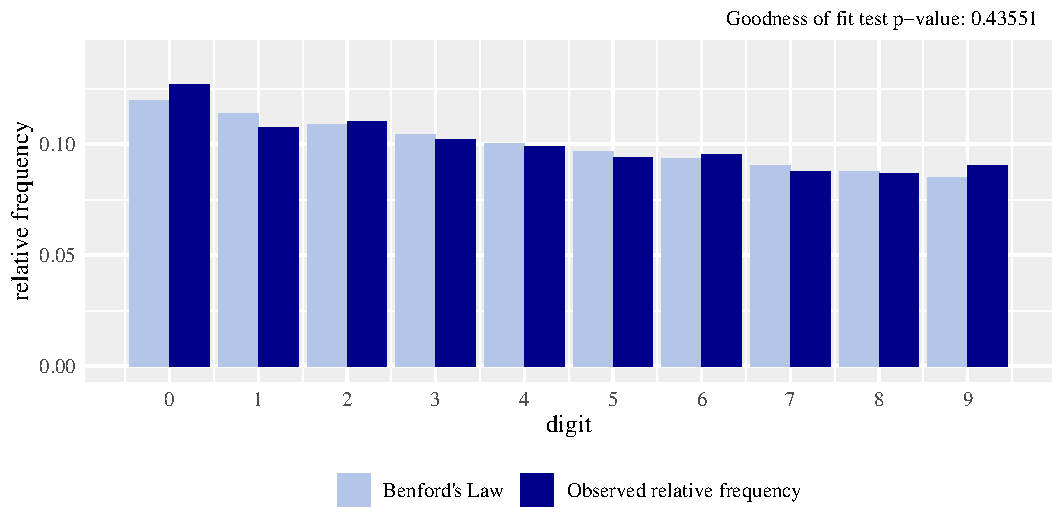
\includegraphics[width=0.99\linewidth]{BT-DT-eng/fig/USA24-both-second_digits.pdf}
%     \label{fig:USA24-both-second_digits}
% \end{figure}

% \begin{figure}[h]
%     \centering
%     \caption{Third digit distribution, total votes, USA 2024}
%     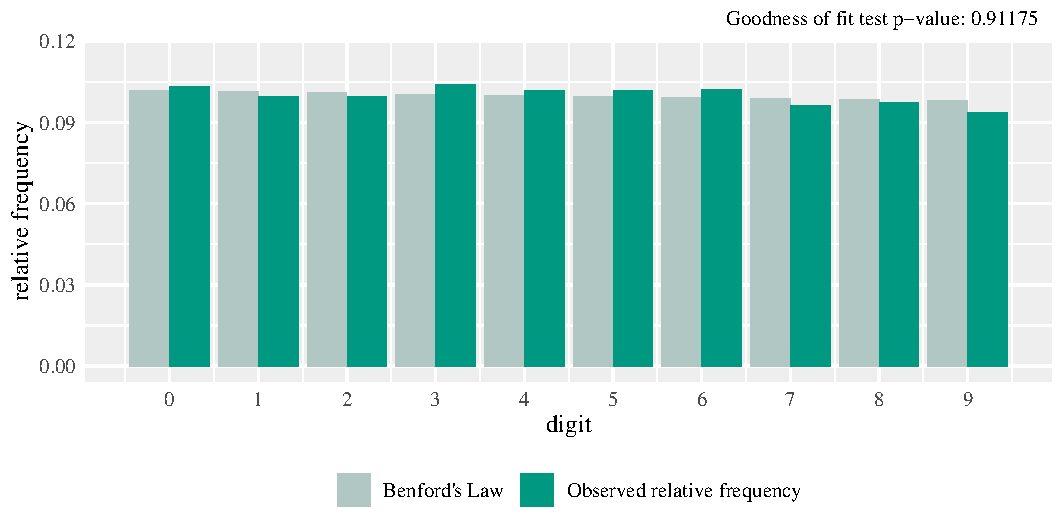
\includegraphics[width=0.99\linewidth]{BT-DT-eng/fig/USA24-both-third_digits.pdf}
%     \label{fig:USA24-both-second_digits}
% \end{figure}

% \begin{figure}[h]
%     \centering
%     \caption{Last digit distribution, total votes, USA 2024}
%     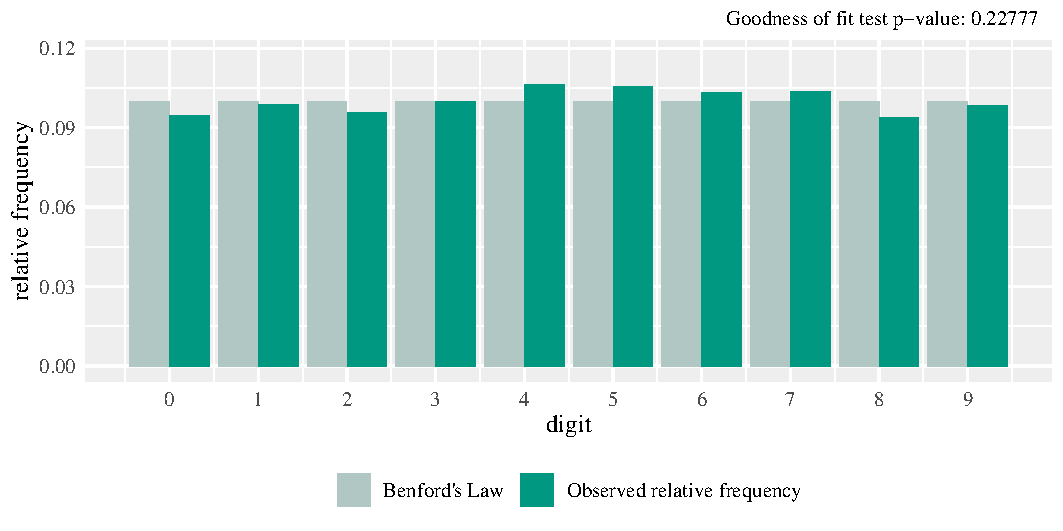
\includegraphics[width=0.99\linewidth]{BT-DT-eng/fig/USA24-both-last_digits.pdf}
%     \label{fig:USA24-both-last_digits}
% \end{figure}

\begin{figure}[h]
    \centering
    \caption{First two digits distribution from both candidates, USA 2024}
    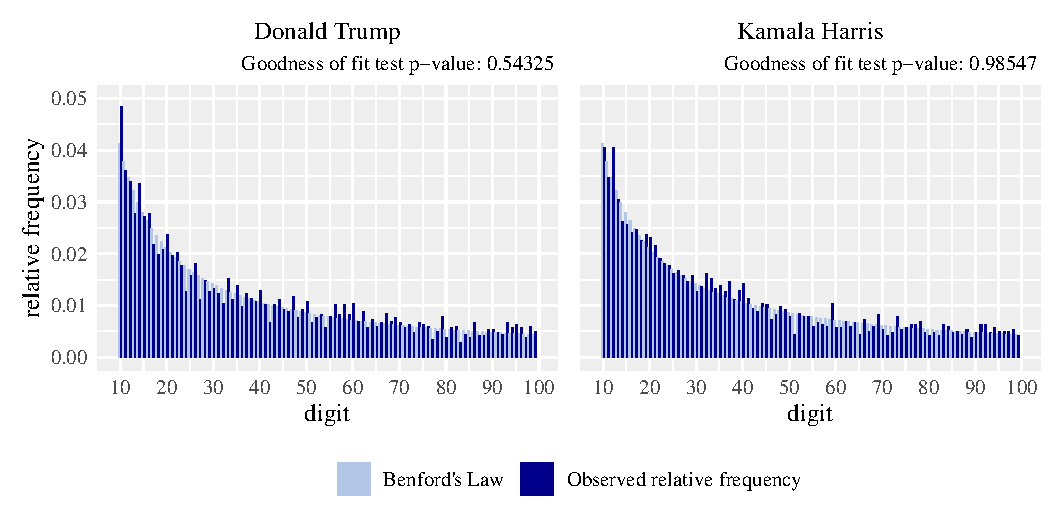
\includegraphics[width=0.99\linewidth]{BT-DT-eng/fig/USA24-dual-first_two_digits.pdf}
    \label{fig:USA24-dual-first_two_digits}
\end{figure}

\begin{figure}[h]
    \centering
    \caption{Third digits distributions from both candidates, USA 2024}
    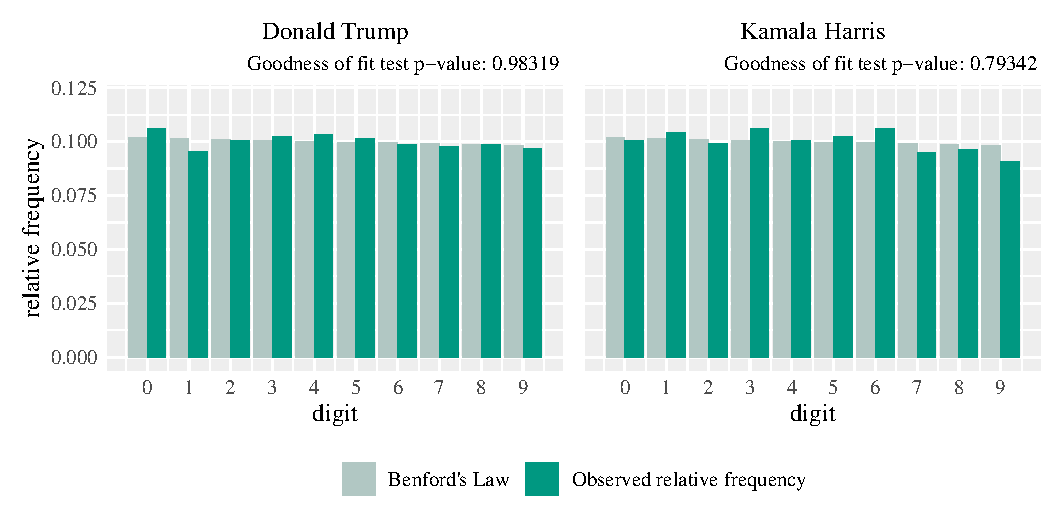
\includegraphics[width=0.99\linewidth]{BT-DT-eng/fig/USA24-dual-third_digits.pdf}
    \label{fig:USA24-dual-third_digits}
\end{figure}








% \include{...}
% \include{...}

\end{document}
